\documentclass[12pt]{article}

\usepackage{amsmath, mathtools}
\usepackage{amsfonts}
\usepackage{amssymb}
\usepackage{graphicx}
\usepackage{colortbl}
\usepackage{xr}
\usepackage{longtable}
\usepackage{xfrac}
\usepackage{siunitx}
\usepackage{tabularx}
\usepackage{float}
\usepackage{booktabs}
\usepackage{caption}
\usepackage{pdflscape}
\usepackage{afterpage}
\usepackage{calc}
\usepackage{multirow}
\usepackage{array}
\usepackage{longtable}
\usepackage{rotating}

\usepackage[a4paper]{geometry}
\usepackage[acronym,nomain,section=subsection,numberedsection]{glossaries}
\usepackage[round]{natbib}
\usepackage[bookmarks=true,breaklinks]{hyperref}

%% Comments

\usepackage{color}

\newif\ifcomments\commentstrue %displays comments
%\newif\ifcomments\commentsfalse %so that comments do not display

\ifcomments
\newcommand{\authornote}[3]{\textcolor{#1}{[#3 ---#2]}}
\newcommand{\todo}[1]{\textcolor{red}{[TODO: #1]}}
\else
\newcommand{\authornote}[3]{}
\newcommand{\todo}[1]{}
\fi

\newcommand{\wss}[1]{\authornote{blue}{SS}{#1}} 
\newcommand{\plt}[1]{\authornote{magenta}{TPLT}{#1}} %For explanation of the template
\newcommand{\an}[1]{\authornote{cyan}{Author}{#1}}

%% Common Parts

\newcommand{\progname}{MECHTRON 4TB6} % PUT YOUR PROGRAM NAME HERE
\newcommand{\authname}{Group 1, UWheeledChair,
\\ Lisa Ji
\\ Haoyu Lin
\\ Yuntian Wang
\\ Zichun Yan } % AUTHOR NAMES                  

\usepackage{hyperref}
    \hypersetup{colorlinks=true, linkcolor=blue, citecolor=blue, filecolor=blue,
                urlcolor=blue, unicode=false}
    \urlstyle{same}
% \hypersetup{
%     colorlinks=true,       % false: boxed links; true: colored links
%     linkcolor=red,          % color of internal links (change box color with linkbordercolor)
%     citecolor=green,        % color of links to bibliography
%     filecolor=magenta,      % color of file links
%     urlcolor=cyan           % color of external links
% }

% For easy change of table widths
\newcommand{\colZwidth}{1.0\textwidth}
\newcommand{\colAwidth}{0.13\textwidth}
\newcommand{\colBwidth}{0.82\textwidth}
\newcommand{\colCwidth}{0.1\textwidth}
\newcommand{\colDwidth}{0.05\textwidth}
\newcommand{\colEwidth}{0.8\textwidth}
\newcommand{\colFwidth}{0.17\textwidth}
\newcommand{\colGwidth}{0.5\textwidth}
\newcommand{\colHwidth}{0.28\textwidth}

\makenoidxglossaries
    \newlength\maxlength
    \newlength\thislength
    \newglossarystyle{mystyle}
    {%
      \renewenvironment{theglossary}%
      {% start of glossary
       % Find maximum width of the first column:
        \setlength{\maxlength}{0pt}%
        \forglsentries[\currentglossary]{\thislabel}%
        {%
           \settowidth{\thislength}{\glsentryshort{\thislabel}}%
           \ifdim\thislength>\maxlength
             \setlength{\maxlength}{\thislength}%
           \fi
        }%
        % Now calculate the width of the second column:
        \settowidth{\thislength}{\hspace{1.5em}=\hspace{1em}}%
        \setlength{\glsdescwidth}{\linewidth-\maxlength-\thislength-2\tabcolsep}%
        % Start the tabular environment
        \begin{tabular}{l@{\hspace{1.5em}=\hspace{1em}}p{\glsdescwidth}}
        \toprule
        \multicolumn{1}{l}{\textbf{symbol}} &
        \multicolumn{1}{@{}l}{\textbf{description}}\\%
        \midrule
      }%
      {% end of glossary
         \bottomrule
         \end{tabular}%
      }%
      % Header has been incorporated into \begin{theglossary}
      \renewcommand*{\glossaryheader}{}%
      % Don't do anything between letter groups
      \renewcommand*{\glsgroupheading}[1]{}%
      \renewcommand*{\glsgroupskip}{}%
      % Set display for each the acronym entry
      \renewcommand{\glossentry}[2]{%
        \glstarget{##1}{\glsentryshort{##1}}% short form
        &
        \glsentrylong{##1}% long form
        \\% end of row
      }%
      % No sub-entries, so \subglossentry doesn't need redefining
    }
\newacronym{wbr}{WBR}{Wheeled Bipedal Robot}
\newacronym{har}{HAR}{Hazard Analysis Report}
\newacronym{imc}{IMC}{Inter-Module Communication}
\newacronym{ca}{CA}{Critical Assumptions}
\newacronym{emi}{EMI}{Electro Magnetic Interference}
\newacronym{imu}{IMU}{Inertial Measurement Unit}
\newacronym{lidar}{LiDAR}{Light Detection and Ranging}
\newacronym{crc}{CRC}{Cyclic Redundancy Check}
\newacronym{srs}{SRS}{System Requirements Specification}
\newacronym{assump}{A}{Assumption}
\newacronym{dd}{DD}{Data Definition}
\newacronym{gd}{GD}{General Definition}
\newacronym{gs}{GS}{Goal Statement}
\newacronym{im}{IM}{Instance Model}
\newacronym{lc}{LC}{Likely Change}
\newacronym{ps}{PS}{Physical System Description}
\newacronym{req}{R}{Requirement}
\newacronym{theo}{T}{Theoretical Model}
\newacronym{macrm}{MacRM}{MacRobomaster Club}
\newacronym{com}{CoM}{Center of Mass}
\newacronym{na}{N/A}{Not Applicable}
\newacronym{dji}{DJI}{SZ DJI Technology Co., Ltd.}
\newacronym{rmul}{RMUL}{RoboMaster University League}
\newacronym{fsm}{FSM}{Finite State Machine}
\newacronym{tbd}{TBD}{To be declared}
\newacronym{pid}{PID}{Proportional–integral–derivative}

\newacronym{uid}{UID}{User Interface Design}
\newacronym{pr}{PR}{Performance Requirements}
\newacronym{cr}{CR}{Communication Requirements}
\newacronym{oer}{OER}{Operational and Environmental Requirements}
\newacronym{msr}{MSR}{Maintainability and Support Requirements}
\newacronym{sr}{SR}{Security Requirements}
\newacronym{ueh}{UEH}{Undesired Event Handling}
\newacronym{no}{NO}{Normal Operation}

% Used so that cross-references have a meaningful prefix
\newcounter{defnum} %Definition Number
\newcommand{\dthedefnum}{GD\thedefnum}
\newcommand{\dref}[1]{GD\ref{#1}}
\newcounter{datadefnum} %Datadefinition Number
\newcommand{\ddthedatadefnum}{DD\thedatadefnum}
\newcommand{\ddref}[1]{DD\ref{#1}}
\newcounter{theorynum} %Theory Number
\newcommand{\tthetheorynum}{T\thetheorynum}
\newcommand{\tref}[1]{T\ref{#1}}
\newcounter{tablenum} %Table Number
\newcommand{\tbthetablenum}{T\thetablenum}
\newcommand{\tbref}[1]{TB\ref{#1}}
\newcounter{assumpnum} %Assumption Number
\newcommand{\atheassumpnum}{P\theassumpnum}
\newcommand{\aref}[1]{A\ref{#1}}
\newcounter{goalnum} %Goal Number
\newcommand{\gthegoalnum}{P\thegoalnum}
\newcommand{\gsref}[1]{GS\ref{#1}}
\newcounter{instnum} %Instance Number
\newcommand{\itheinstnum}{IM\theinstnum}
\newcommand{\iref}[1]{IM\ref{#1}}
\newcounter{reqnum} %Requirement Number
\newcommand{\rthereqnum}{P\thereqnum}
\newcommand{\rref}[1]{R\ref{#1}}
\newcounter{lcnum} %Likely change number
\newcommand{\lthelcnum}{LC\thelcnum}
\newcommand{\lcref}[1]{LC\ref{#1}}

\title{System Requirements Specification\\\progname}
\author{\authname}
\date{\today}

\begin{document}

\maketitle
\pagenumbering{arabic}

\newpage
\begin{table}[hp]
    \caption{Revision History} \label{TblRevisionHistory}
    \begin{tabularx}{\textwidth}{llX}
        \toprule
        \textbf{Date} & \textbf{Developer(s)}    & \textbf{Change} \\
        \midrule
        2023-11-10    & Lisa Ji, Haoyu Lin       & Revision 0      \\
                      & Yuntian Wang, Zichun Yan &                 \\
        \bottomrule
    \end{tabularx}
\end{table}

\newpage
\tableofcontents
\newpage
\listoftables
\listoffigures

\newpage
\section{Introduction}
This document provides an overview of the \acrfull{srs} for the UWheeledChair project of Group 1.
\subsection{Project Purpose} \label{sec:Project Purpose}
\begin{figure}[H]
    \centering
    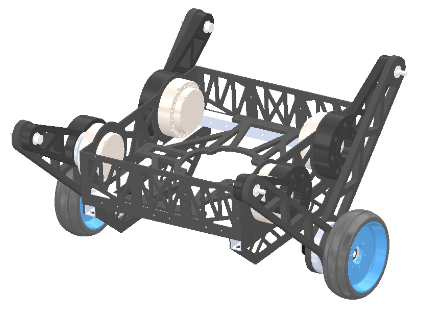
\includegraphics[scale=0.7]{../Mechanical Platform.png}
    \caption{\acrshort{wbr} Mechanical Platform}
    \label{fig:Mechanical Platform}
\end{figure}
This project is to develop the software and control system for a fully-autonomous delivery robot, based on the existing assembly of a \acrfull{wbr} provided by the \acrfull{macrm}, as shown in Figure \ref{fig:Mechanical Platform}. The project will be referred to as the \acrshort{wbr} project in the following documents.\\\\
For \acrshort{macrm}, \acrshort{wbr} was constructed following the constraints defined in the rules, \citet{RmuBuildSpecs2024}, of the 2024 \acrfull{rmul} Competition, whose host is \acrfull{dji}. Details of the constraints is shown in section \ref{sec:Design Constraints}.\\\\
Since the mechanical and electronic hardware are fixed constraints, the \acrshort{wbr} project mainly focuses on the software and control system, while the \acrshort{macrm} is responsible for the mechanical design, provision, and maintenance.
\subsection{Document Purpose}
The purpose of this document is to locate a full range of system requirements for the development of a \acrshort{wbr}. It encompasses a broad spectrum of aspects, including general behaviors, functional breakdown, and in-depth performance criteria. It delves into strategies for addressing unforeseen circumstances and the likelihood of changes in these requirements. It also acts as a benchmark to evaluate whether the future design meets all specified requirements.
\subsection{Organization of Document}
This document is a modified Volere template as in \cite{RobertsonAndRobertson2012} and has been adopted according to project needs. The document follows the general organization of the Volere template with some additional sections to better suit for Mechatronics. It contains scope of the requirements and overview of system behaviours, which gives readers general concept of what are contained in this document. The performance requirements are separated into two parts, functional and nonfunctional. Referring to different requirements, the normal operation and undesired event handling are covered. The likelihood of Each requirement is determined. This allows readers to follow a flow from general to specific details for the system requirements of \acrshort{wbr}.\\
Neglected subsections from the Volere template are: the hands-on users of the product, persona, priorities assigned to users, users participation, maintenance users and service technicians,implementation environment of the current system, partner or collaborative applications, off-the-shelf software, anticipated workplace environment, enterprise constrains, relevant facts, business rule.
\subsection{The Stakeholders}
\subsubsection{The Client}
\begin{itemize}
    \item Dr.Alan Wassyng, Professor from McMaster University, Computing and Software Department.
    \item \acrfull{macrm}, a robotics engineering club of McMaster University
\end{itemize}

\subsubsection{The Customers}
\begin{itemize}
    \item People who wants to save time moving objects over a moderately long distance and moderately complex terrain.
    \item People who requires unmanned transportation of goods over a moderately long distance and moderately complex terrain.
    \item People who requires secured transportation of goods over a moderately long distance and moderately complex terrain.
\end{itemize}

\subsubsection{Other Stakeholders}
\acrshort{na}


\section{Design Constraints} \label{sec:Design Constraints}
\subsection{Mechanical Platform}
As mentioned in section \ref{sec:Project Purpose}, the \acrshort{wbr} is constrained by the rules of 2024 \acrshort{rmul}. From page 26 to 27 of the robot specification manual, \citet{RmuBuildSpecs2024}, our "Balancing Standard Robot" is constrained to have all ground-contacting surfaces aligned on the same line and cannot keep balance without dynamic adjustment. Additionally, to win the competition, the robot shall be light, fast, robust, and small.\\\\
\begin{figure}[H]
    \centering
    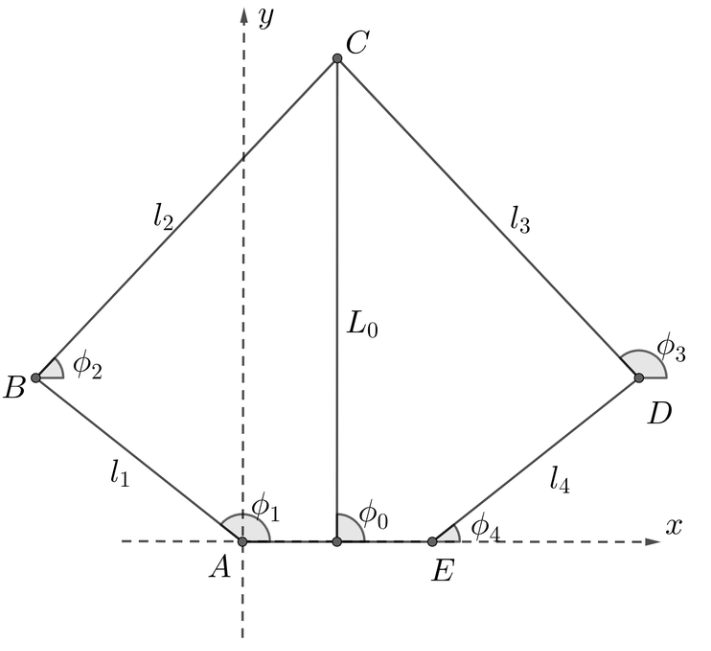
\includegraphics[scale=0.5]{../Leg Linkage.png}
    \caption{Sketch of \acrshort{wbr} Leg Linkage, from \citet{HarbinEngCtrlDesign2022}}
    \label{fig:Leg Linkage}
\end{figure}
Therefore, \acrshort{macrm} decided to put a five-bar linkage configuration on per side of the \acrshort{wbr}, by following the paper \citet{WbrBalanceControl2021}. Shape of each linkage, as illustrated in figure \ref{fig:Leg Linkage}, is controlled by a pair of two hip-joint motors, which changes the overall robot posture as a result. The two motors contacting the ground are drive motors, which regulates the horizontal movement.
\subsection{Electronic Platform}
\acrshort{macrm} designed the electronic system according to the rules of \acrshort{rmul} as shown in figure \ref{fig:WBR Electronic System}. The rationale of choice of each specific component is out of scope of this document.
% \begin{figure}[H]
\begin{sidewaysfigure}
    \centering
    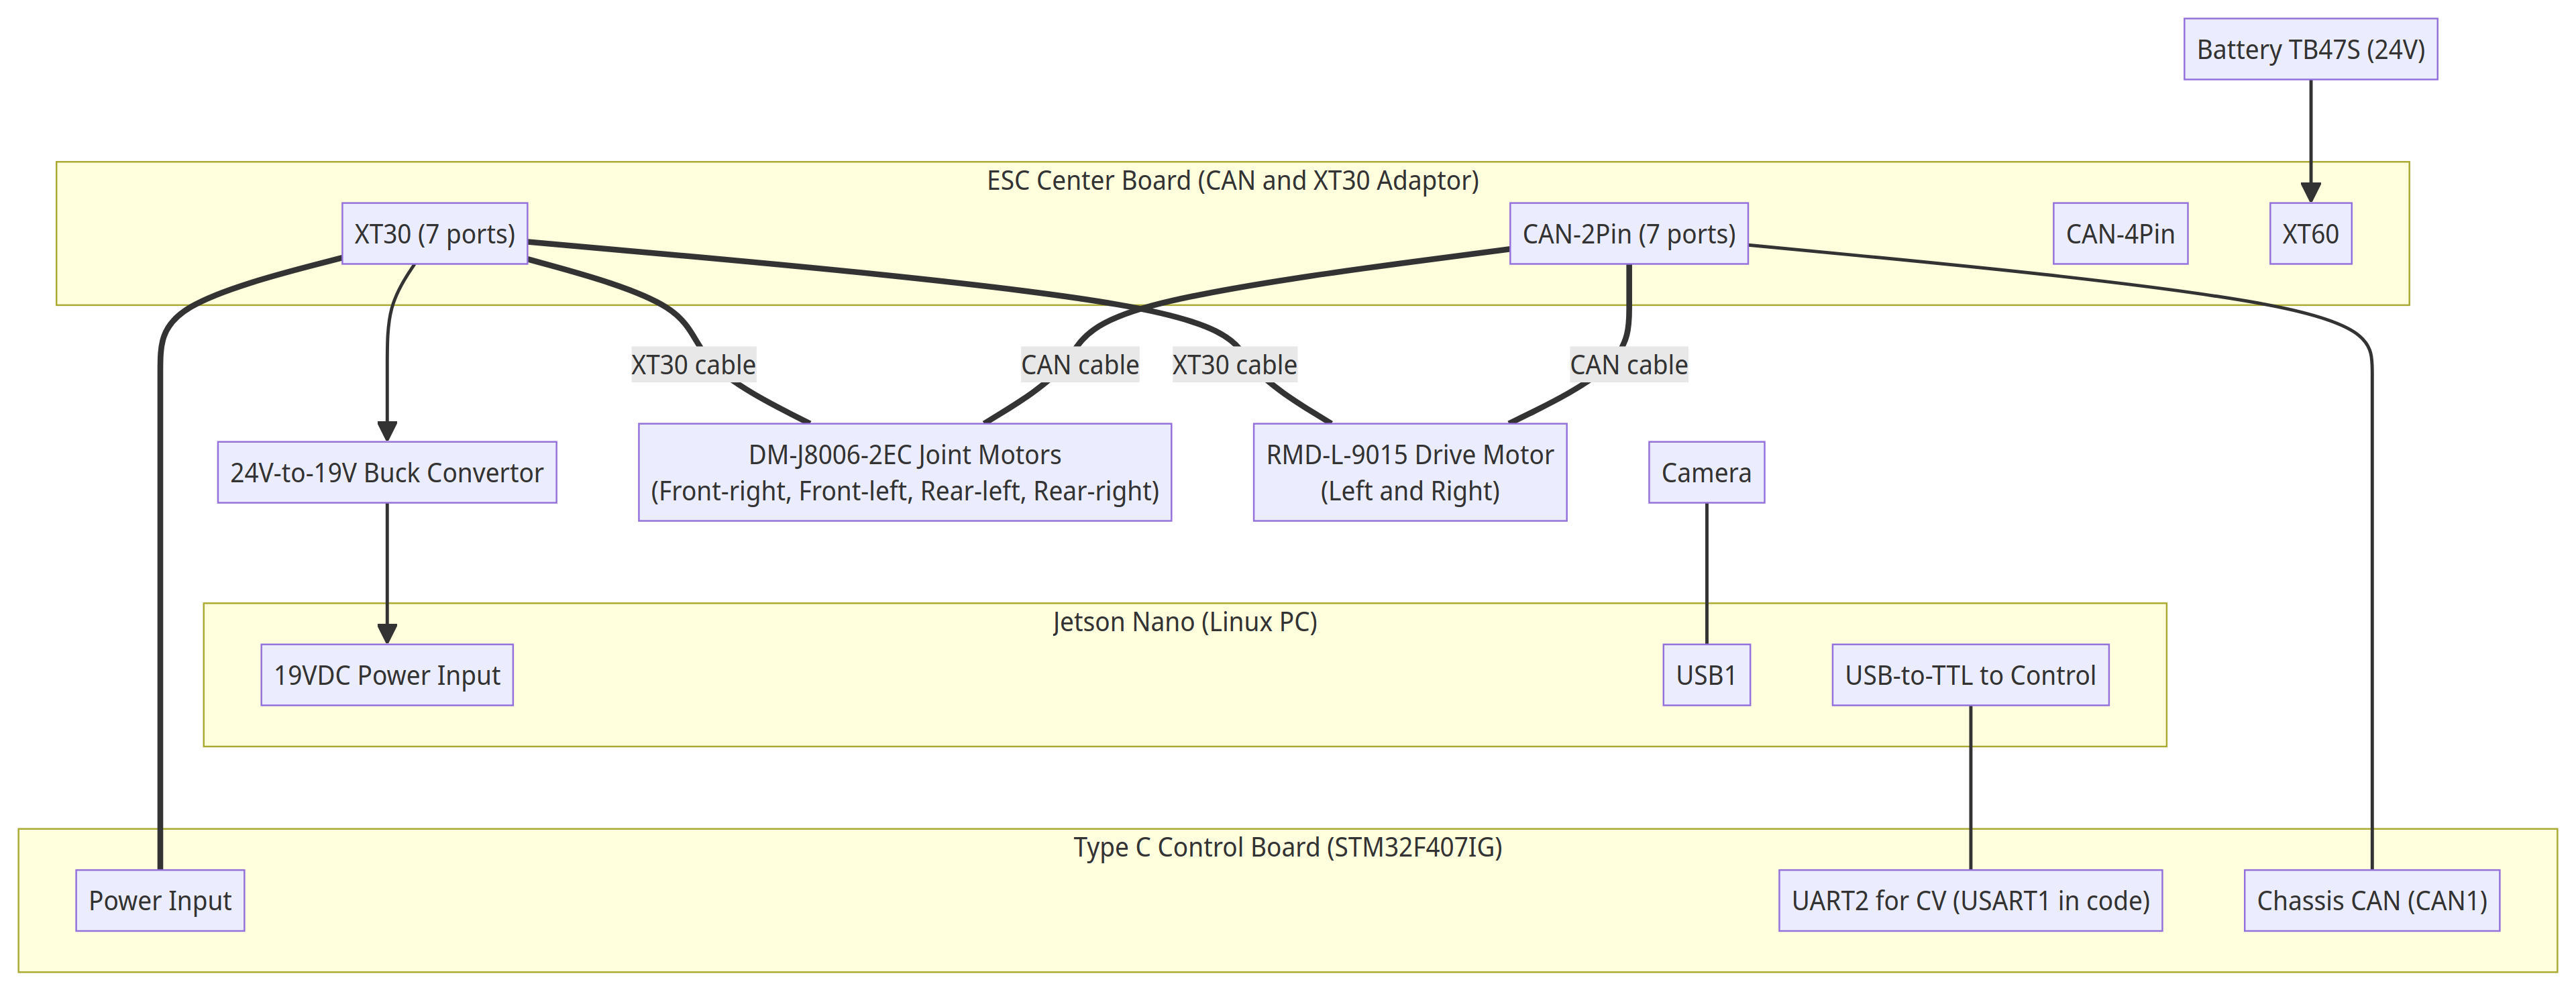
\includegraphics[width=\textwidth,height=\textheight,keepaspectratio]{../Electronic System Diagram.png}
    \caption{WBR Electronic System}
    \label{fig:WBR Electronic System}
% \end{figure}
\end{sidewaysfigure}
% \end{landscape}

\section{Project Constraints}
\subsection{Mandated Constraints}
\begin{center}
    \begin{tabular}{|| p{3cm} || p{8cm} ||}
        \hline
        MC1         & The complete project design needs to be done by the end of academic year                                                                        \\
        \hline
        Description & Based on the course outline, the deadline of the capstone project is by the end of the academic year                                            \\
        \hline\hline
        MC2         & The cost of the whole project should not exceed \$750                                                                                           \\
        \hline
        Description & There is a budgetary constraint on this project to deter individuals from acquiring pre-packaged "solutions."                                   \\
        \hline\hline
        MC3         & The design should be a combination of software and hardware.                                                                                    \\
        \hline
        Description & As a hard requirement for all Mechatronics groups, the design must encompass not only software components but also integrate hardware elements. \\
        \hline\hline
    \end{tabular}
\end{center}

\subsection{Relevant Facts and Assumptions}
\subsubsection{User Characteristics}
Users of the \acrshort{wbr} are anticipated to have specific demands related to object delivery. These users might lack the time to personally handle deliveries or seek to allocate time to more crucial tasks. Additionally, the \acrshort{wbr} suits individuals who facing mobility challenges. Users are expected to possess fundamental knowledge of controlling the robot's movement through the use of a remote control unit, enabling them to interact effectively with the technology.
\subsubsection{Reader Characteristics}
The potential readers of this document comprises technicians and individuals with engineering backgrounds or a keen interest in robotic designs.
Given the technical nature of the content, readers are expected to possess some professional knowledge and understanding in both hardware and software fields. Familiarity with the engineering design process is crucial to facilitate comprehension and navigation through the document. This feature enables efficient searching, allowing readers to locate their relevant area of interest promptly without the need to invest time in comprehending the entire document.This technical resource is also open to enthusiastic learners without prior engineering knowledge. Rationales are provided where concepts may be challenging, enabling readers to follow and understand the content effectively.

\subsubsection{Assumptions and Dependencies}
\label{sec:Assumptions and Dependencies}
\textbf{AD1:} The user should be capable of visually tracking or observing the robot's movements with their eyes. \\
\textbf{Rationale:} In order to control the movement of the robot, the user should have a basic idea where the robot goes and what its destination is, so they can monitor the robot's path or ensure it navigates as intended.\\\\
\textbf{AD2:} Assuming that users interacting with the robot have a basic understanding of how to control it using a remote control unit. \\\\
\textbf{AD3:} Assuming the robot works within a predetermined and specified environmental conditions.\\
\textbf{Rationale:} The extreme weather, such as -30 degree celsius condition would prevent the robot from working normally. Therefore, assuming it is placed in moderate working conditions.


\section{Scope}
\subsection{Scope of Requirements}
The responsibilities of the stakeholders and the \acrshort{wbr} are as follows:
\begin{itemize}
    \item Package Sender Responsibilities: The Package Sender is responsible to provide appropriate inputs and environment to the system as mentioned in the relevant parts of \nameref{sec:Assumptions and Dependencies}. % @TODO: change to specific AD
    \item Package Receiver Responsibilities: The Package Receiver is responsible to provide appropriate inputs to the system as mentioned in the relevant parts of \nameref{sec:Assumptions and Dependencies}. % @TODO: change to specific AD
    \item \acrshort{wbr} Responsibilities: The \acrshort{wbr} provides suggestion of paths to reach the target location and let Package Sender choose the path to go; determines the robot's intended routes and desired motions; It processes data received from sensors, which detect obstacles and unfamiliar terrain. The motor system primarily handles the robot's mechanical movements.
\end{itemize}

\subsection{The Scope of the Work}
\subsubsection{The Context of the Work}
\begin{figure}[H]
    \centering
    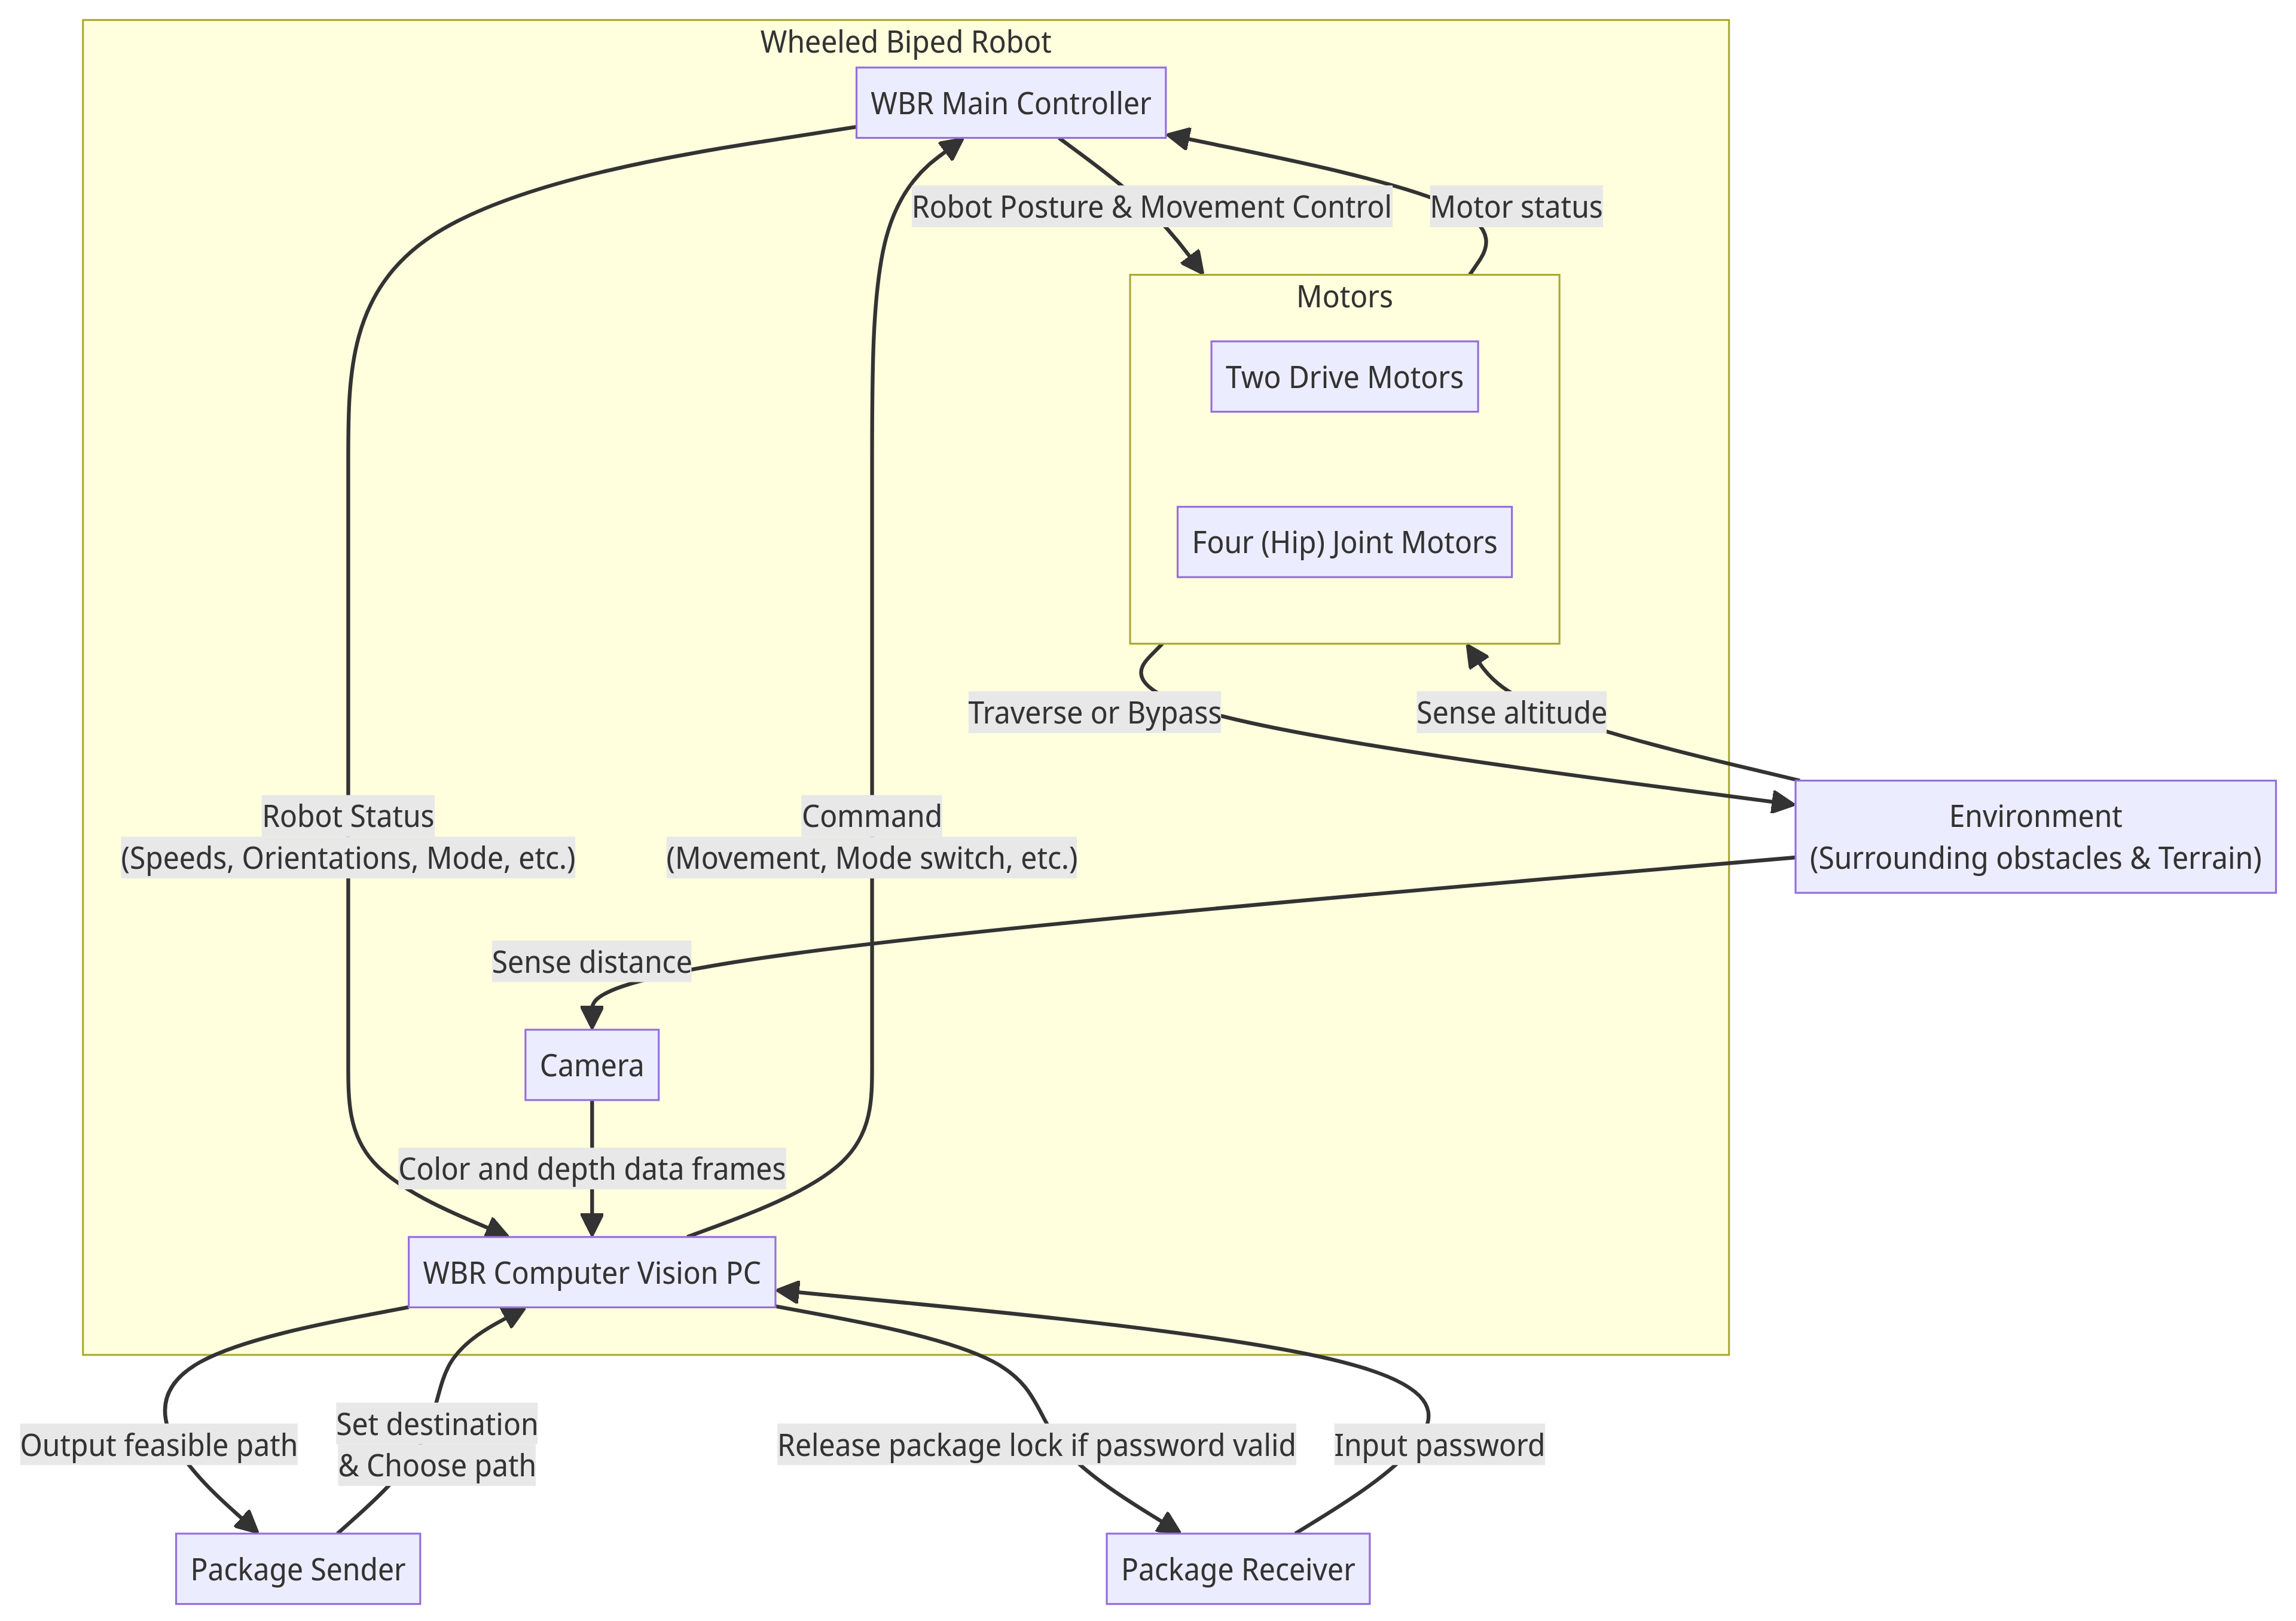
\includegraphics[width=\textwidth,height=\textheight,keepaspectratio]{../System Context Diagram.png}
    \caption{System Context Diagram}
\end{figure}
The following picture shows the design of the context diagram of the project, it illustrates the core interaction between the \acrshort{wbr} and its immediate external entities. In this diagram, the \acrshort{wbr} is the central system, the information regarding the condition of the environment is detected, such as the distance from the nearest obstacle, then the \acrshort{wbr} takes the reaction on how to handle a certain situation. The package sender acts as the external entity, it sets the destination and picks a route for the \acrshort{wbr} and the \acrshort{wbr} provides it the feasible path and goes to complete the package delivery. The package receiver is another external entitle, it inputs password, in response to it, the \acrshort{wbr} releases the package once it confirms the validity of the password.
\begin{figure}[H]
    \centering
    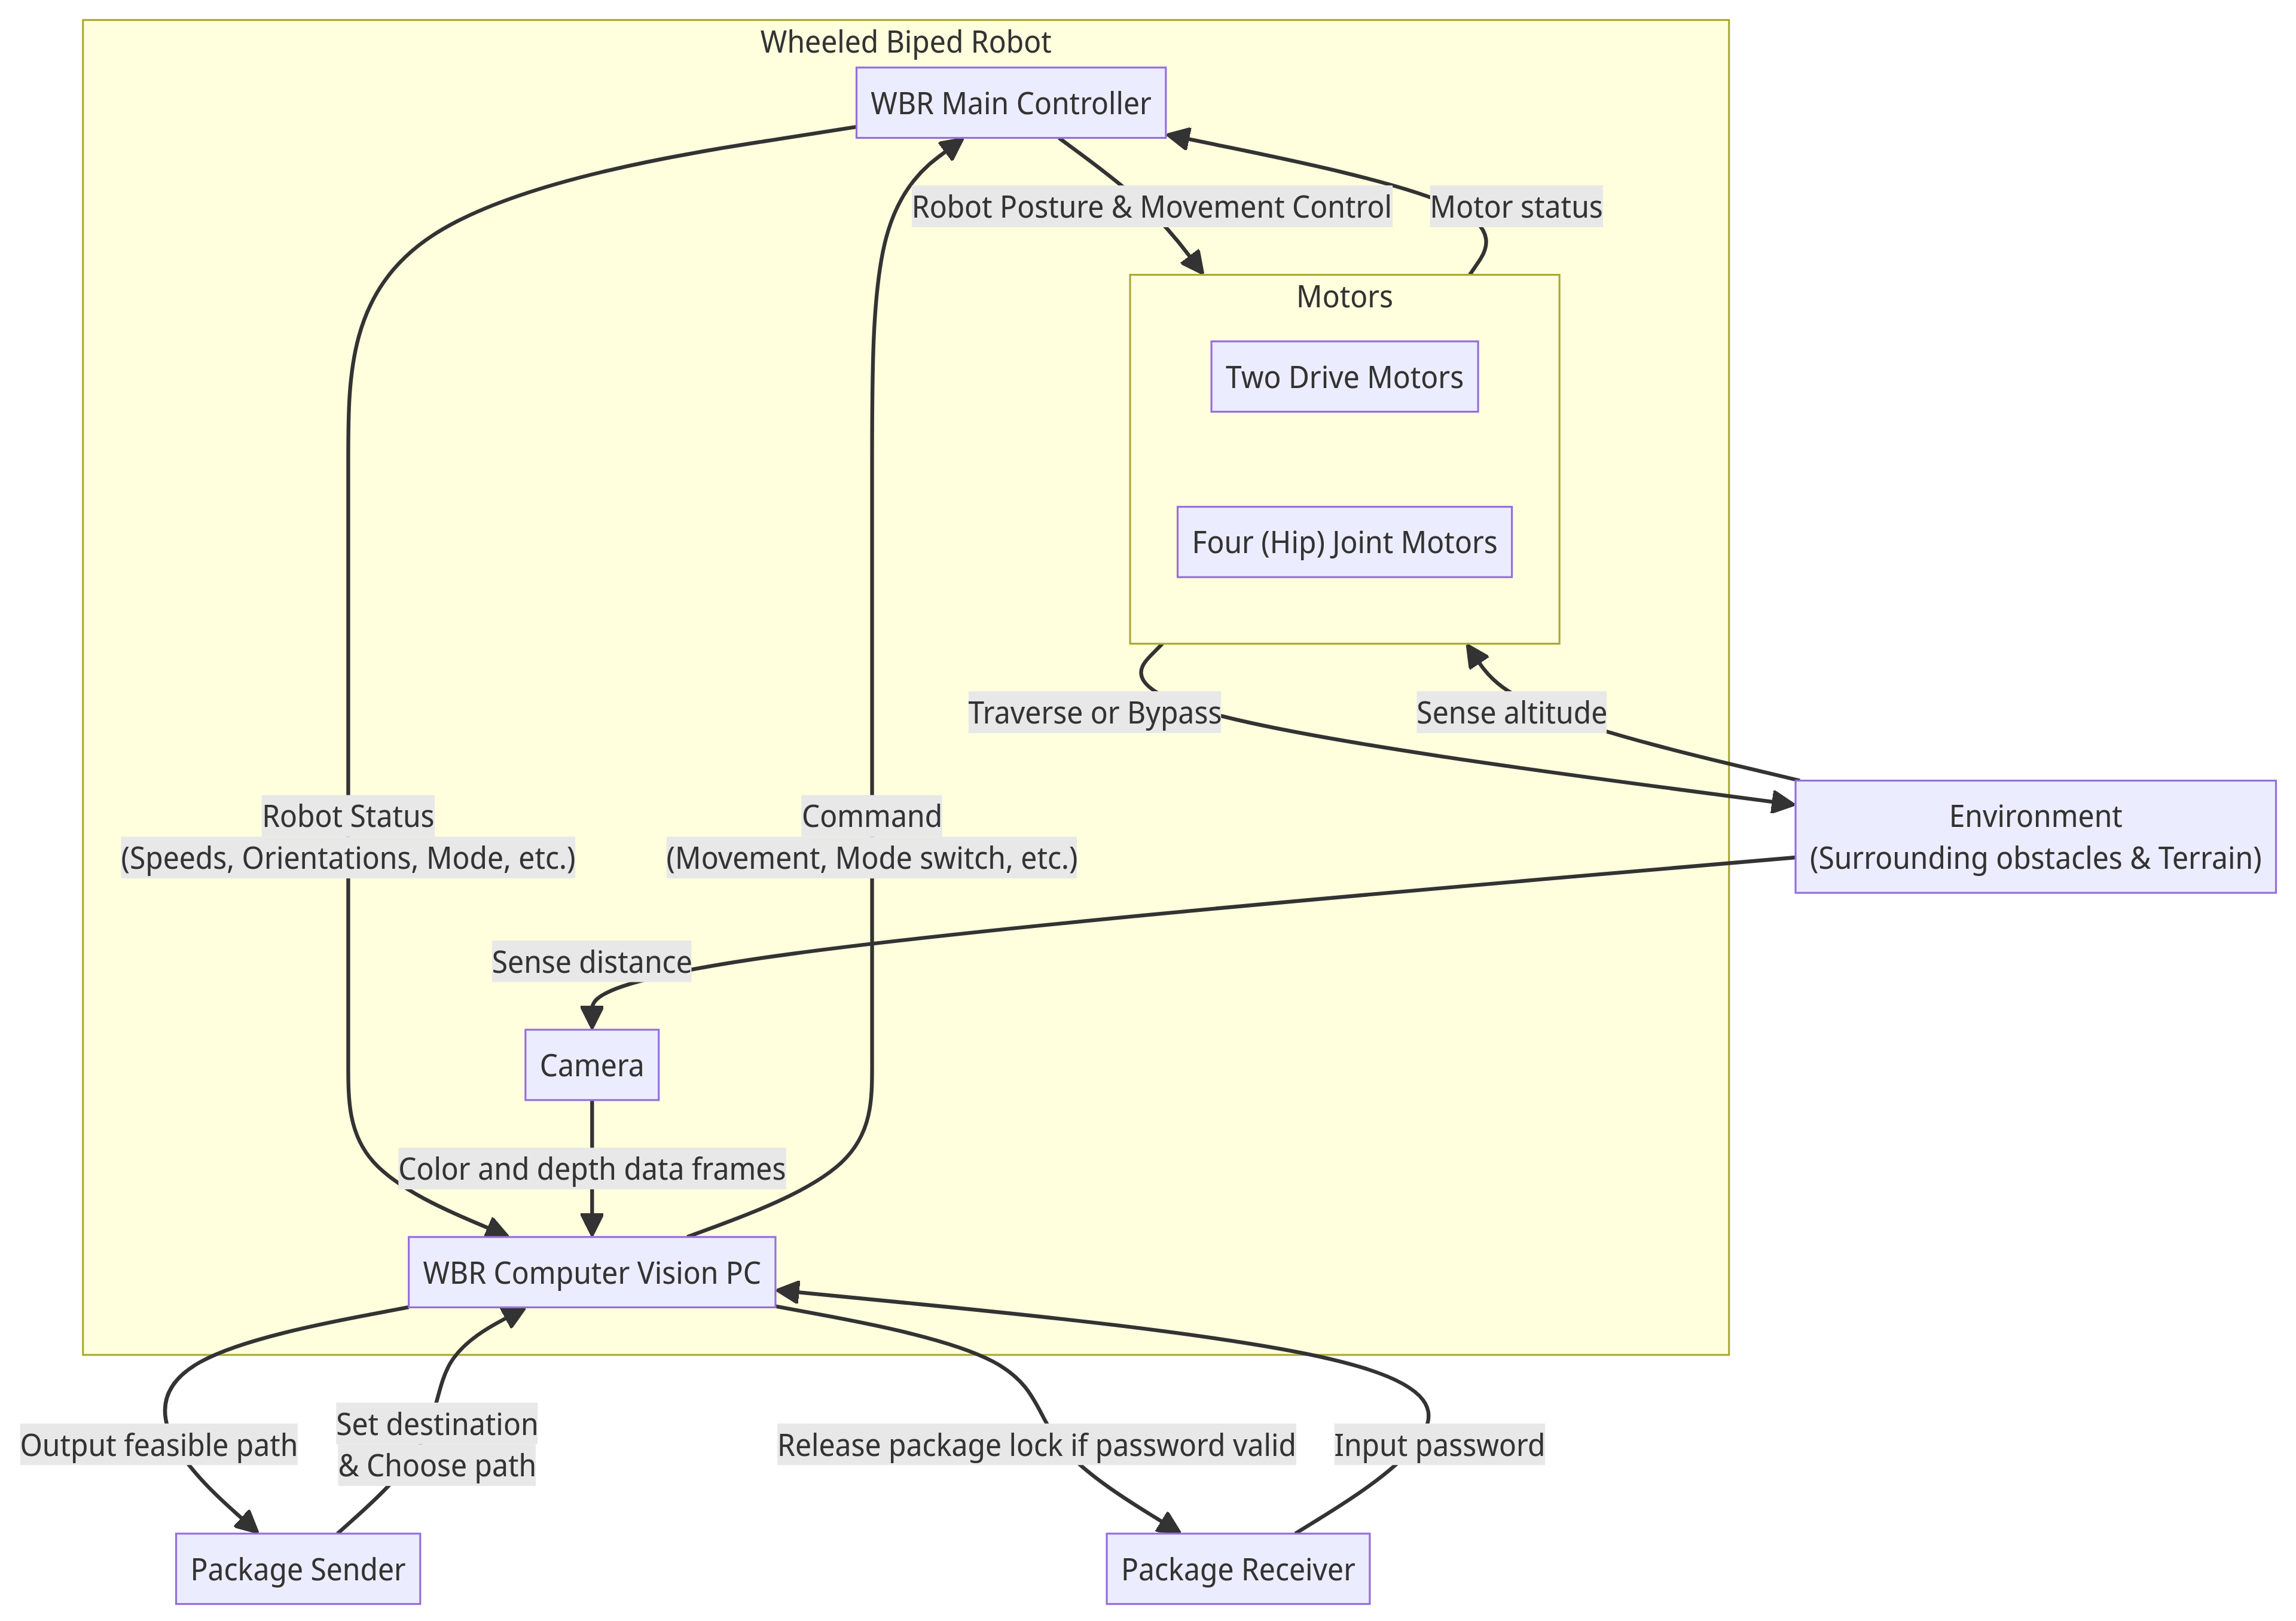
\includegraphics[width=\textwidth,height=\textheight,keepaspectratio]{../Complete System Diagram.png}
    \caption{Complete System Diagram}
\end{figure}


\section{Behaviour Description}
To make the behaviour of the product to achieve the target task, the Finite State Machine is created to describe the behaviour with detailed description provided after the picture.
\begin{figure}[H]
    \centering
    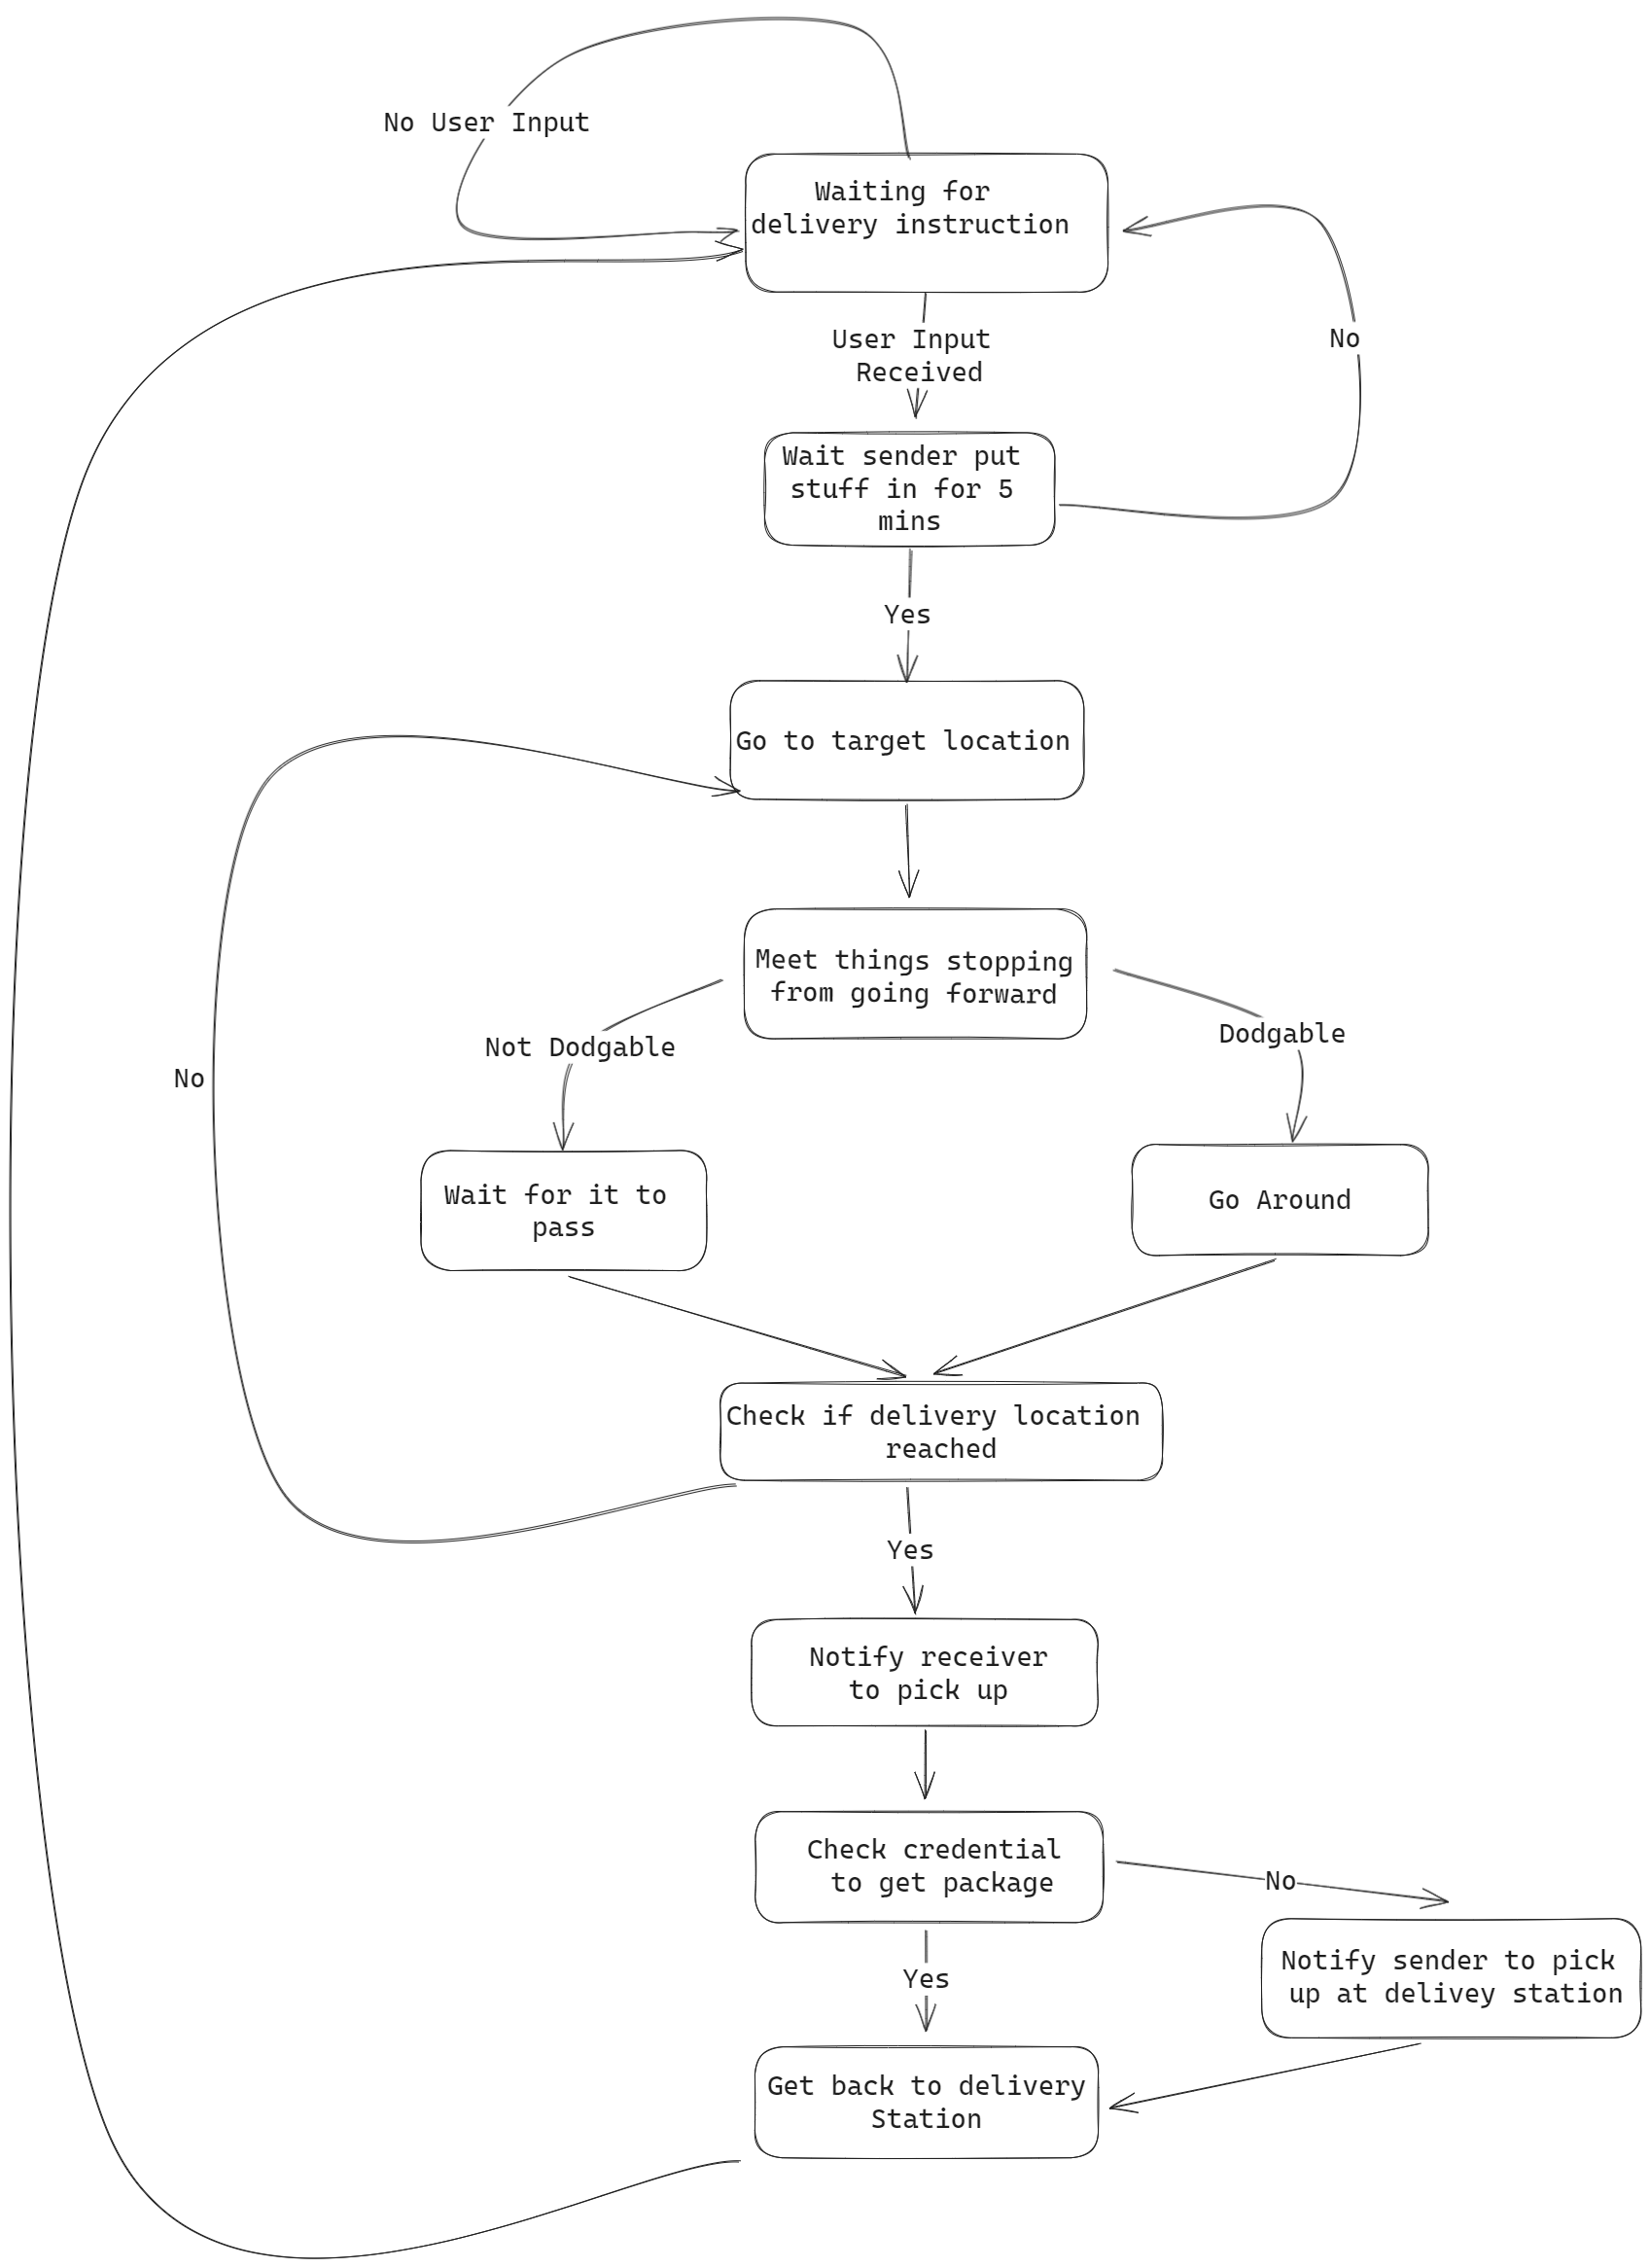
\includegraphics[width=\textwidth,height=\textheight,keepaspectratio]{../state-machine.png}
    \caption{System Behaviour Finite State Machine}
\end{figure}

\subsection{State Transition Descriptions}
The Finite State Machine diagram briefly introduces the following general behaviours state. The description is given below:\\\\
\noindent\textbf{Waiting for delivery instruction:} It will need to stay in the delivery station to wait for new delivery instructions coming in from a client \\\\
\noindent\textbf{Wait sender put stuff in for 5 mins:} Upon receiving a  delivery instruction, the robot initiates waiting status to allow sender side client to put stuff in delivery box for 5 mins. If there is nothing inside after 5 mins, it will return back the first status to waiting next delivery instruction\\\\
\textbf{Go to target location:} After sender side client put stuff in for delivery. Robot will start navigation to the target location. \\\\
\textbf{Meet things stopping from going forward :} When the sensor detects nearby obstacles, it communicates this information to the control system. The system temporarily interrupts the ongoing path travel task and initiates the execution of a special task.\\\\
\textbf{Check if delivery location reached:} When going closer to the delivery location or algorithm detect \acrshort{wbr} reached target destination. It will go check if it actually reached or not.\\\\
\textbf{Notify Reciver to pick up :} After comfirming the target destination is reached, \acrshort{wbr} will notify Reciver to pick package up. \\\\
\textbf{Check credential to get package :} This status will ensure only the person will credential can get the package, other wise it will bring the package back to original delivery station.  \\\\
\textbf{Get back to delivery Station :} After finishing delivery task, it will go back to delivery station for next delivery task or wait there until previous failed delivery to be pick up. \\\\


\subsection{State Behaviour Description and Rationales}
\noindent\textbf{Waiting for delivery instruction:}When the \acrshort{wbr} is positioned in delivery Station, in the absence of any initial user commands, it enters an "Idle" state. During this state, the robot's motor system is powered on, and the robot readies itself to receive and respond to user commands once they are initiated. .  \\\\
\noindent\textbf{Wait sender put stuff in for 5 mins:} 5 mins is a reasonable length to detect if client has put stuff in or not. If there is already stuff in, \acrshort{wbr} will stay in unavailable status until it being picked up by either client or MacRM.  \\\\
\textbf{Go to target location:} This is the starting state for delivery navigation. Once \acrshort{wbr} enter this status. It means it is in delivery process now.  \\\\
\textbf{Meet things stopping from going forward :} This status has 2 solution, one is wait until the object go away and one is finding a workaround. Since we do not want the robot just to stand at 1 position for whole day. That is the reason why we will have a timeout as well for waiting. \\\\
\textbf{Check if delivery location reached:} This status is to check if the algorithm working alright on \acrshort{wbr}. We will have at at least 3 ways to decide if robot reach the destination or not. \\\\
\textbf{Notify Receiver to pick up :} This action is to make sure the receiver knows \acrshort{wbr} is there and will be notify to avoid missing delivery.  \\\\
\textbf{Check credential to get package :} This state will make sure that package is delivered to the correct person.  \\\\
\textbf{Get back to delivery Station :} This is the final status of \acrshort{wbr} delivery task. Since it need to go back to the delivery station whatever it finished delivery or not(if receiver didn't pick it up in certain amount of time).\\\\


\subsection{Jump Behaviour}
The figure \ref{fig:Jump FSM} shows the whole process of jump action of WBR, including the process before it receives the jump command and after if fully completes the jump action and resumes initial position.
\begin{figure}[H]
    \centering
    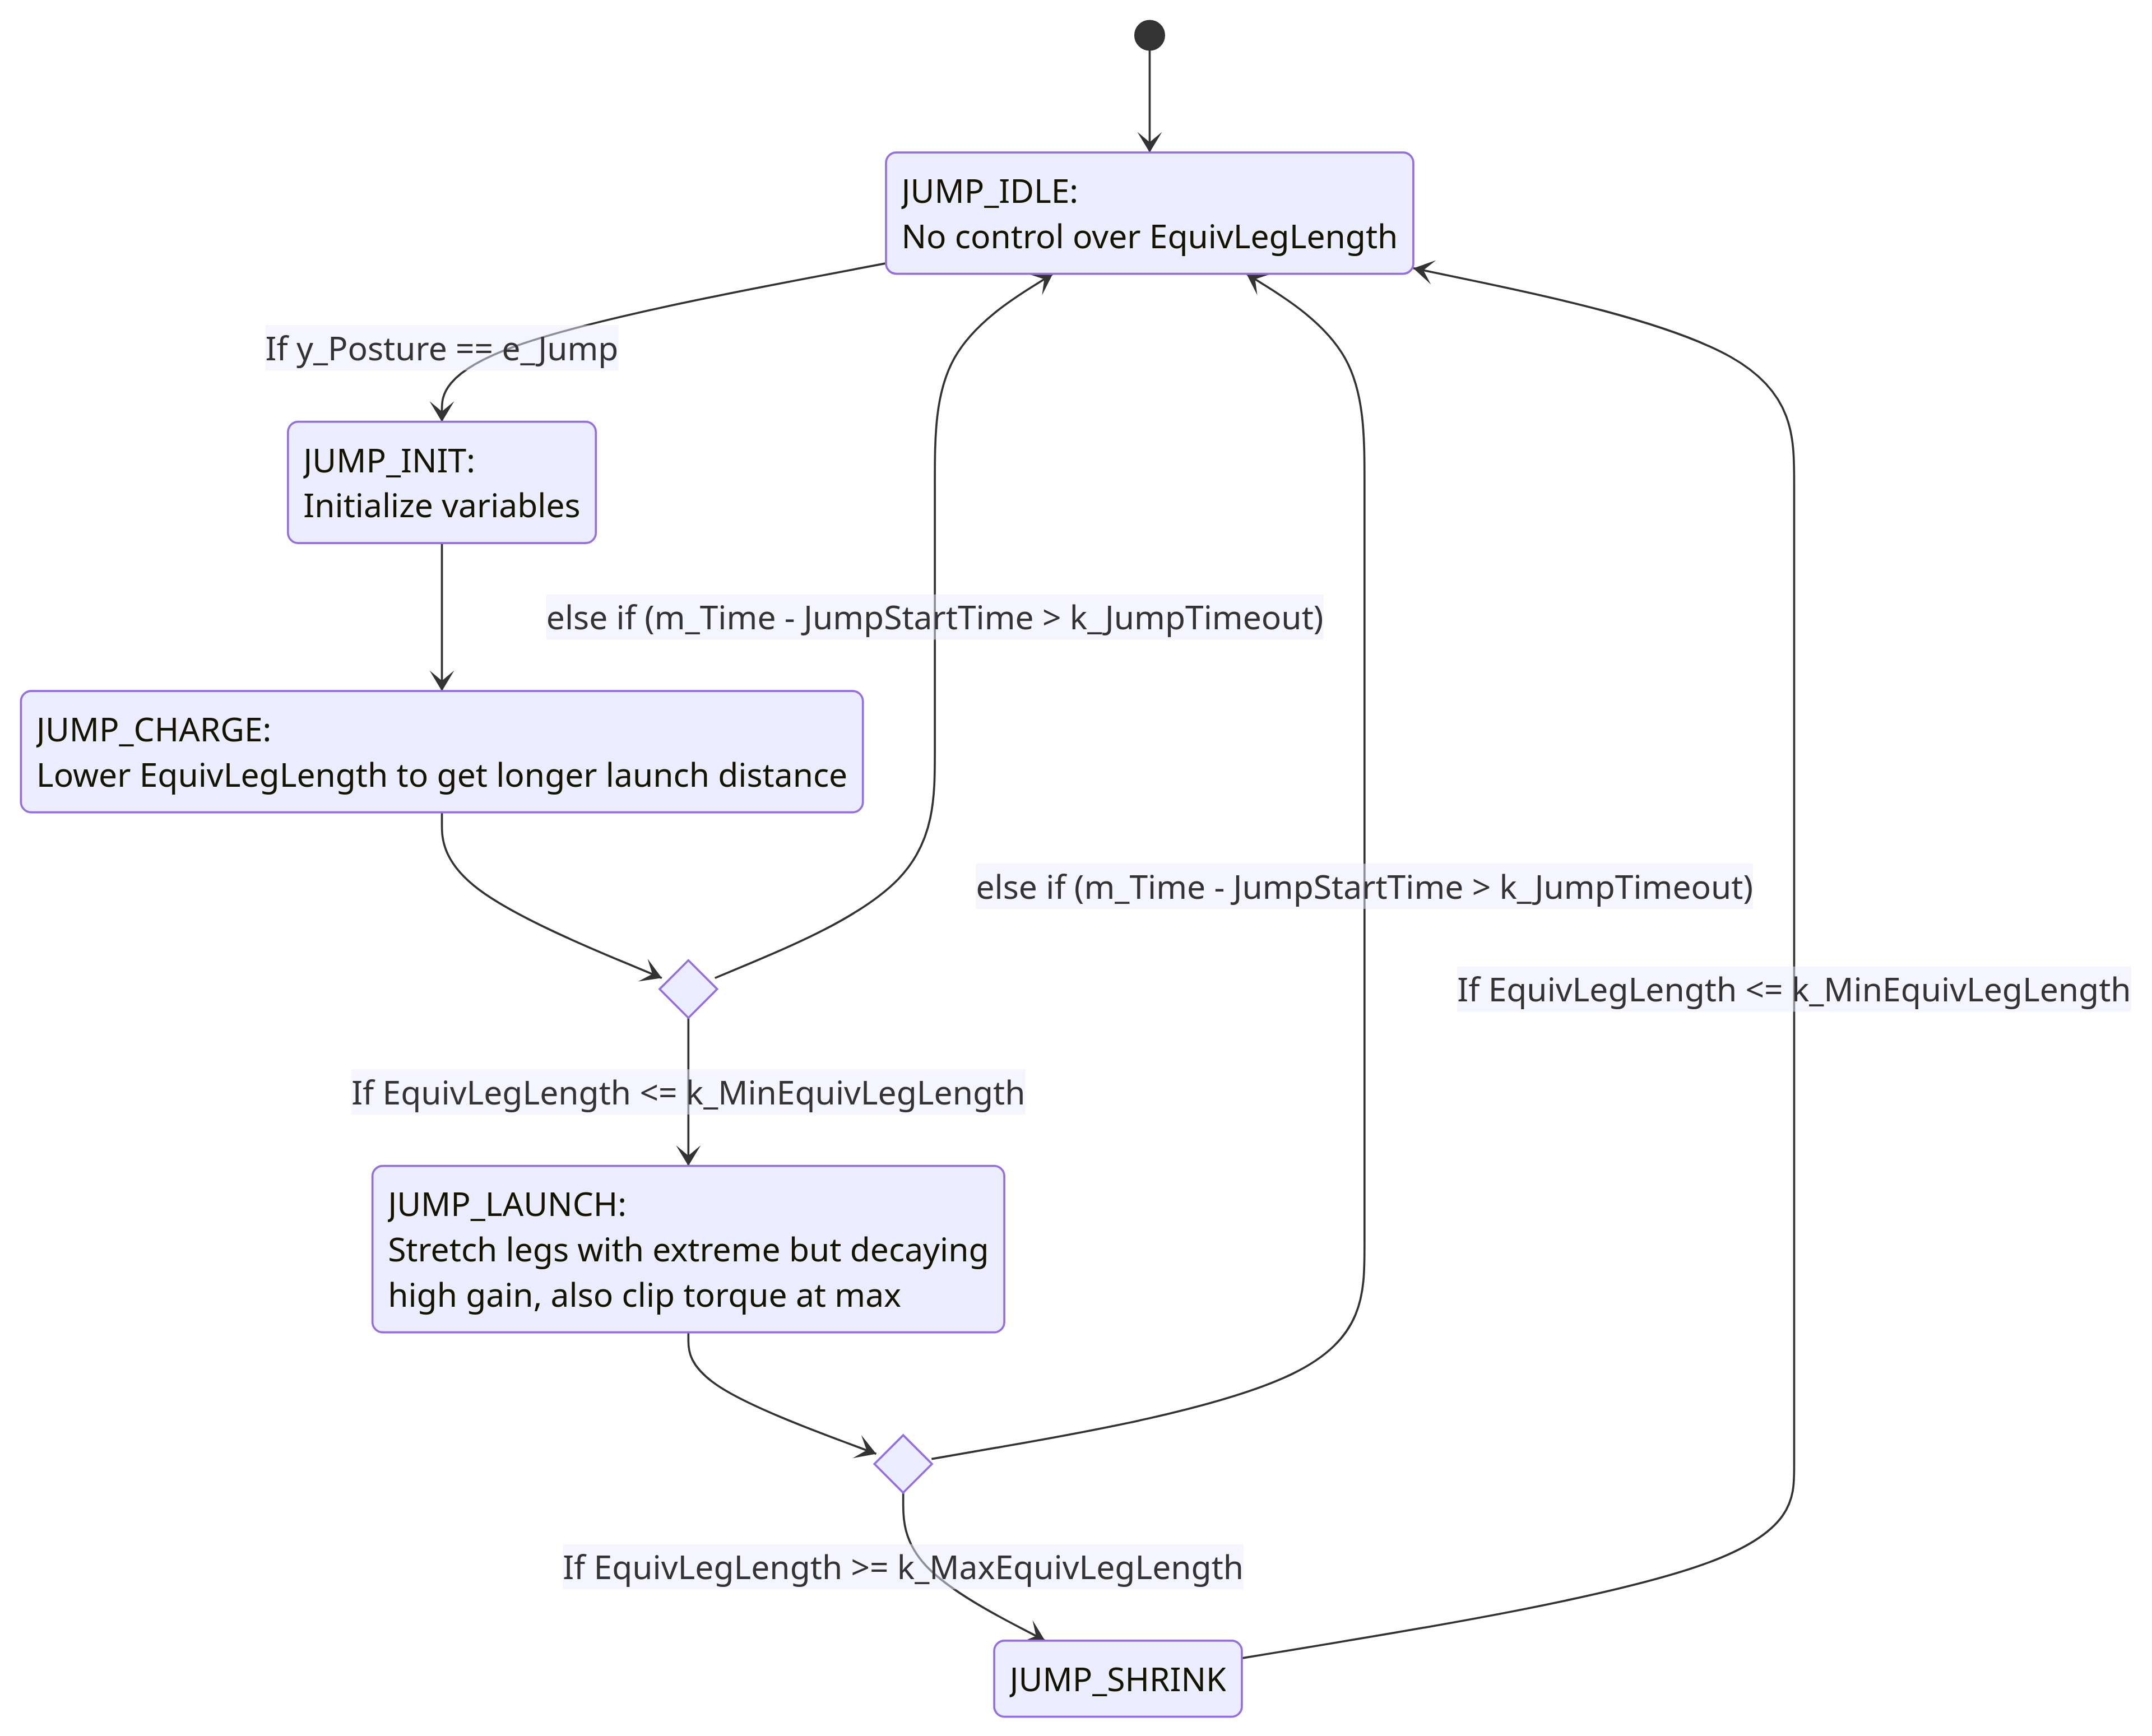
\includegraphics[width=\textwidth,height=\textheight,keepaspectratio]{../Jump FSM.png}
    \caption{Jump \acrshort{fsm}}
    \label{fig:Jump FSM}
\end{figure}

\subsubsection{State Descriptions}
\textbf{JUMP\_IDLE:} WBR stays idle when there is no command received.\\\\
\textbf{JUMP\_CHARGE:} WBR lower the \acrshort{com} to a predetermined level for the purpose of getting a longer launch distance. This primarily aimed at accumulating more energy for a higher jump. It is important to ensure CoM remains within the robot's bearing capacity, and it should not exceed the lowest acceptable CoM level.\\\\
\textbf{JUMP\_LAUNCH:} Stretching legs but with decaying gain. The intentional reduction in gain serves as a buffer, mitigating large torques to prevent potential damage to the components.\\\\
\textbf{JUMP\_SHRINK:} Lower CoM to its initial position.\\\\


\section{Functional Requirements}
The following are the functional requirements of the project. They are separated into 2 main parts: robot mobility and environment sensing.
Note: All monitored, controlled variables and constants can be found in section \ref{sec:VARIABLES MASTER LIST}.
\subsection{Functional Decomposition and Work Partitioning}
\begin{sidewaysfigure}
    \centering
    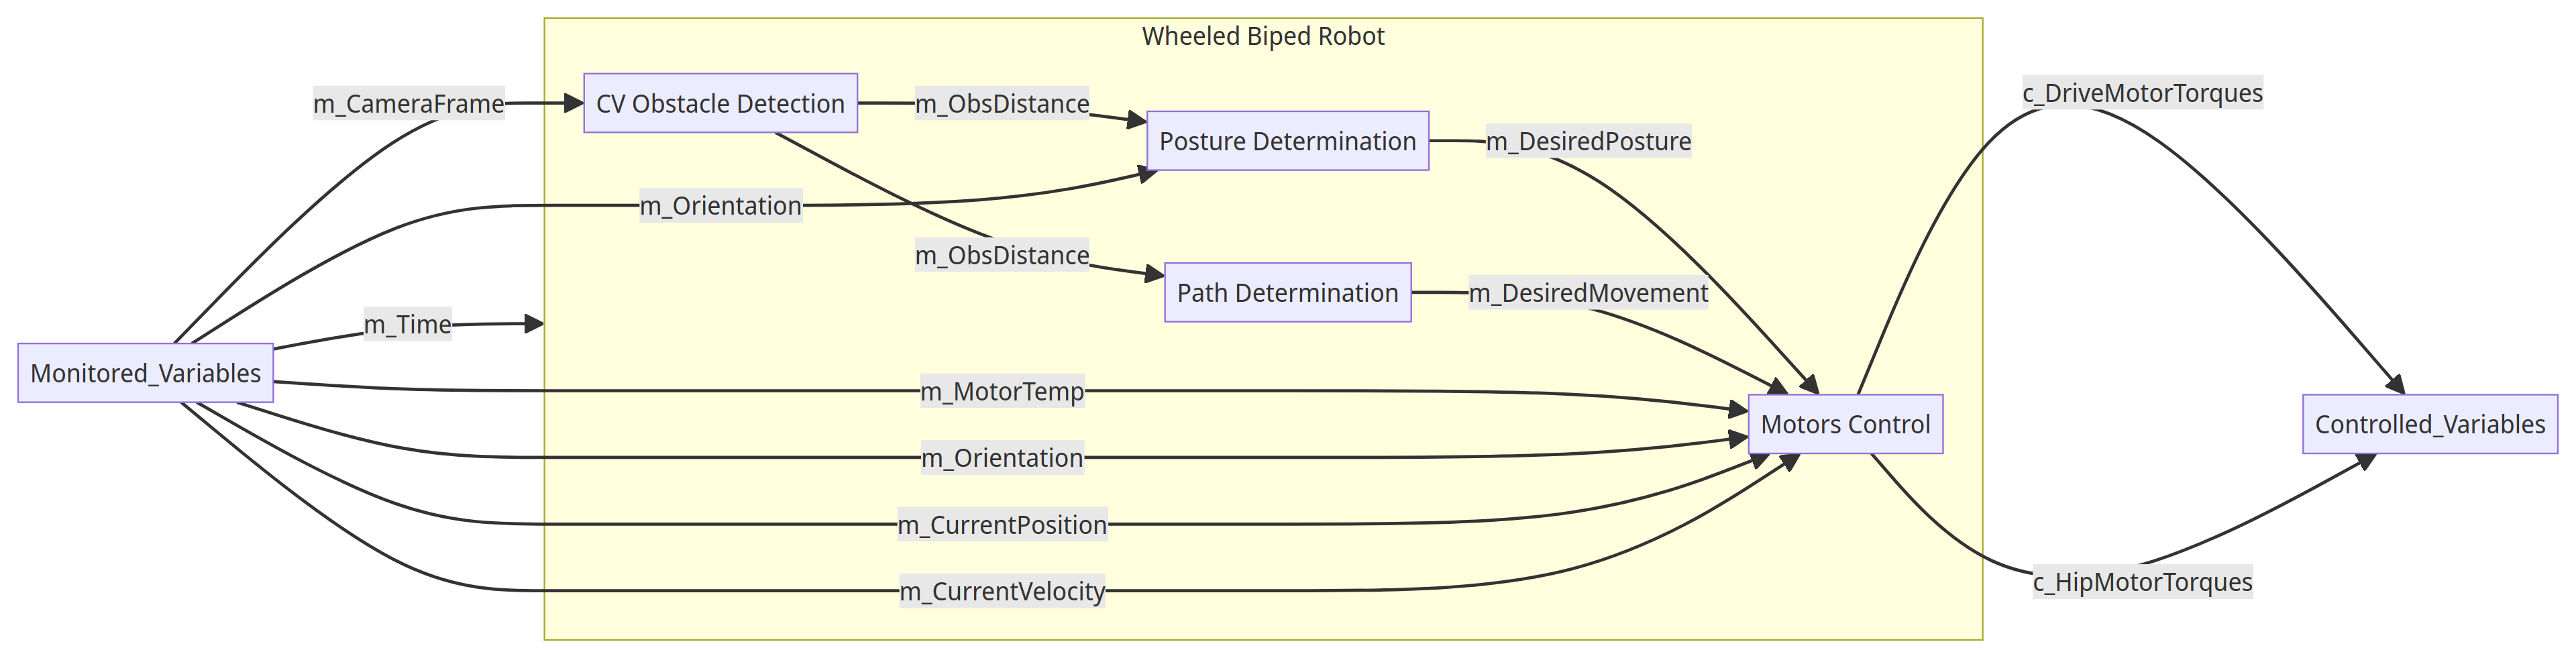
\includegraphics[width=\textwidth,height=\textheight,keepaspectratio]{../Function_Decom.png}
    \caption{Functional Decomposition Diagram} \label{lbl:Function_Decom}
\end{sidewaysfigure}
The following table shows the work partitioning of the project. It lists all possible events taking place during the operation of the \acrshort{wbr}. The functional decomposition diagram is also attached as figure \ref{lbl:Function_Decom}.

\begin{table}[H]
    \caption{Work Partitioning}
    \begin{tabularx}{\textwidth}{|p{3cm}|X|X|}
        \toprule
        \textbf{Event Name} & \textbf{Input} & \textbf{Output}                         \\
        \midrule
        CV Obstacle Detection               & Depth and colour data frame from camera  & Characteristic distances to major obstacles, e.g. perpendicular distance to walls. \\
        \hline
        Posture Determination & Current chassis orientation; distances to nearby obstacles that reduces safe workspace. & Desired posture as joint configurations. \\
        \hline
        Path Determination & distances to nearby obstacles that eliminates alternative routes to go & Desired horizontal velocity including rotational and translational velocity. \\
        \hline
        Motors Control & Motor feedback data, Chassis orientation, and desired robot kinematics & Desired torques of all motors. The integrated motor controller hardware will ensure the torque further. \\
        \bottomrule
    \end{tabularx}
\end{table}

\textbf{Trigger conditions}:
\begin{itemize}
    \item \textbf{Path Determination Event: }Triggered when the system determines the optimal path for the wheeled biped robot based on various inputs, including obstacle detection and posture determination.
    \item \textbf{Motors Control Event: } Involves the control of motors to execute movements, influenced by the desired path, posture, and obstacle detection.
    \item \textbf{Obstacle Detection Event: } Activated when the system detects obstacles in the robot's path, influencing the path determination and motors control processes.
    \item \textbf{Posture Determination Event: } Occurs when the system determines the optimal posture or position for the robot, affecting the motors control process.
    \item \textbf{Input Update Event: } Involves updating the input parameters, including obstacle information, orientation, current position, and current velocity of the robot.
    \item \textbf{Desired Path Update Event: } Triggered when the system updates the desired path based on various factors, including obstacle detection and the current posture.
    \item \textbf{Jump State Event: } Activated when the system encounters a condition requiring to jump, influencing the posture determination process.
    \item \textbf{Position Update Event: } Involves updating the current position of the robot, impacting the motors control process.
    \item \textbf{Velocity Update Event: } Occurs when the system updates the current velocity of the robot, influencing the motors control process.
    \item \textbf{Output Generation Event: } Involves generating output parameters, including position, velocity, and acceleration, which are sent as commands to the WBR.
\end{itemize}

\subsection{Robot Mobility}
\noindent\textbf{RM1:} The \acrshort{wbr} must be capable of moving smoothly and without jerky motions in various directions, including forward, backward, left, right, and rotation.\\
\noindent\textbf{Rationale:}  Seamless movement ensures the \acrshort{wbr}'s agility and adaptability in unpredictable environments, promoting efficient navigation and minimizing disturbances for improved overall performance and user experience.\\

\noindent\textbf{RM2:} The robot should be able to follow the command from Computer Vision board to go through unpredictable environments with obstacles of varying sizes and shapes. It must react to command fast. \\
\noindent\textbf{Rationale:} Since the control board for \acrshort{wbr} movement is separated from the path finding and tracking one which process all the data from sensor. So the control board need to react fast enough to the command passing from Computer Vision board \\

\noindent\textbf{RM3:} The robot should maintain stability while moving on uneven terrain and when transitioning between different types of surfaces, such as from smooth floors to rough terrain.\\
\noindent\textbf{Rationale:} The stability requirement ensures the \acrshort{wbr}'s capability to navigate diverse environments safely, mitigating the risk of instability during transitions between surfaces.\\

\noindent\textbf{RM4:} The robot's average speed should be at most 5m/s when navigating through typical outdoor environments. The maximum speed for safety should not exceed that.\\


\subsection{Environment Sensing}
\noindent\textbf{ES1:} The robot must detect obstacles in its path using LiDAR, cameras, or other methods. It should identify obstacles at least 2 meters before reaching them.\\

\noindent\textbf{ES2:} The robot should be able to sense the environment, including changes in elevation, and surface irregularities, to give out command accordingly.\\

\noindent\textbf{ES3:} The robot should be able to recognize and differentiate between various objects in its environment, such as people, furniture, and other potential obstacles.\\
\noindent\textbf{Rationale:} The ability for object recognition is crucial as it enables the robot to distinguish between diverse environmental elements, enhancing navigation precision and enabling informed decision-making to navigate safely through varied scenarios.\\



\section{Nonfunctional Requirements}
The next paragraphs will talk about about non-functional requirements in the designing of the \acrshort{wbr}, which will be discussed in several different parts.
\subsection{Look and Feel Requirements}
\textbf {\acrshort{na}}

\subsection{Usability and Humanity Requirements}
\subsubsection{User Interface Design}

\noindent\textbf{\acrshort{uid}1:} The robot's user interface should be designed with simplicity and clarity, ensuring operators can easily understand and navigate controls without extensive training or guidance.\\

\noindent\textbf{UID2:}  The robot's control interface should support customization to accommodate users with different physical and cognitive abilities.\\

\subsection{Performance Requirements}
\noindent\textbf{\acrshort{pr}1:}  The robot should maintain optimal performance on various terrains, including smooth floors and rough outdoor environments.\\

\noindent\textbf{PR2:}  Control system's response time to Computer Vision Board commands should be within 0.2s to ensure real-time interaction.\\

\noindent\textbf{PR3:}  The robot should be highly reliable, with a low probability of system failures or malfunctions during operation\\

\noindent\textbf{PR4:}  The robot should be able to withstand minor collisions or impacts without sustaining significant damage that would impair its performance.\\

\subsection{Operational and Environmental Requirements}
\noindent\textbf{\acrshort{oer}1:} The robot should able to operate within normal weather condition. \\
\subsubsection{Communication Requirements}
\noindent\textbf{\acrshort{oer}2:} The robot should be capable of establishing and maintaining wireless communication with external systems for data transfer.\\


\subsection{Maintainability and Support Requirements}
\noindent\textbf{\acrshort{msr}1:} The robot should support remote diagnostics, allowing maintenance teams to identify and address issues without physical intervention.\\
\noindent\textbf{MSR2:} The software should be easily upgradable, enabling the implementation of new features and improvements as technology advances.\\

\subsection{Security Requirements}
\noindent\textbf{\acrshort{sr}1:} The robot's control systems should implement authentication mechanisms to prevent unauthorized access, ensuring secure and controlled operation.\\
\noindent\textbf{SR2:} The robot must have an emergency stop mechanism that can be activated to halt all movements in case of an imminent collision or other safety concerns.\\
\noindent\textbf{SR3:} The robot should be equipped with mechanisms or sensors to prevent tipping over when navigating uneven or inclined terrain.\\


\section{Durability and Reliability}
\noindent\textbf{Operating Time:} The robot should be capable of continuous operation for at least 20 mins before requiring recharging or maintenance.\\
\noindent\textbf{Reliability:} The robot should be highly reliable, with a low probability of system failures or malfunctions during operation.\\
\noindent\textbf{Robustness:} The robot should be able to withstand minor collisions or impacts without sustaining significant damage that would impair its performance.\\

\subsection{Battery Life}
\noindent\textbf{Battery Endurance:} The robot's onboard power source should provide sufficient energy for the robot to operate for at least 5 hours on a single charge.\\
\noindent\textbf{Recharge Time:} The time required for recharging the robot's batteries should not exceed 2 hours to minimize downtime.\\
\subsection{Communication}
\noindent\textbf{Wireless Communication:} The robot should be capable of establishing and maintaining wireless communication with external systems for data transfer.\\

\subsection{Safety}
\noindent\textbf{Emergency Stop:} The robot must have an emergency stop mechanism that can be activated to halt all movements in case of an imminent collision or other safety concerns.\\
\noindent\textbf{User Interface:} The robot should have a user interface that reject suspicious behavior.\\
\noindent\textbf{Hit prevent:} The robot should have soft material surround it to prevent undesired behavior damaging any surrounding.\\

\subsection{Compliance}
\noindent\textbf{Regulatory Requirements:} The robot's performance should comply with all relevant safety and regulatory standards for robotics in the intended operating environment.




\section{Traceability and Priority}
For both functional and non-functional requirements, the dependency matrix is made and priorities are assigned to each requirement. The Traceability matrix and priority table are shown below. In addition, the likelihood change of the requirements and the future plan of the requirements are also shown below.

\subsection{Requirement Matrix}
\begin{table}[H]
    \begin{tabular}{|p{0.45\textwidth}| p{0.45\textwidth}|}

        \hline Functional Requirement ID & Nonfunctional Requirement ID \\

        \hline RM1                       & UID1                         \\

        \hline RM2                       & UID2                         \\
        \hline RM3                       & PR1                          \\
        \hline RM4                       & PR2                          \\
        \hline ES1                       & PR3                          \\
        \hline ES2                       & PR4                          \\
        \hline ES3                       & OER1                         \\
        \hline                           & CR1                          \\
        \hline                           & MSR1                         \\
        \hline                           & MSR2                         \\
        \hline                           & SR1                          \\
        \hline                           & SR2                          \\
        \hline                           & SR3                          \\


        \hline
    \end{tabular}
    \caption{Requirement Traceability Matrix}
\end{table}

\subsection{Priority Table}
\begin{table}[H]
    \begin{tabular}{|p{0.36\textwidth}|p{0.42\textwidth}|p{0.1\textwidth}|}
        \hline Functional Requirement ID & Nonfunctional Requirement ID & Priority \\
        \hline RM1                       &                              & HIGH     \\
        \hline RM2                       &                              & HIGH     \\
        \hline RM3                       &                              & HIGH     \\
        \hline RM4                       &                              & HIGH     \\
        \hline ES1                       &                              & HIGH     \\
        \hline ES2                       &                              & HIGH     \\
        \hline ES3                       &                              & HIGH     \\
        \hline                           & SR1                          & HIGH     \\
        \hline                           & SR2                          & HIGH     \\
        \hline                           & SR3                          & HIGH     \\
        \hline                           & UID1                         & MED      \\
        \hline                           & UID2                         & MED      \\
        \hline                           & PR1                          & MED      \\
        \hline                           & PR2                          & MED      \\
        \hline                           & PR3                          & MED      \\
        \hline                           & PR4                          & MED      \\
        \hline                           & OER1                         & HIGH     \\
        \hline                           & CR1                          & MED      \\
        \hline                           & MSR1                         & MED      \\
        \hline                           & MSR2                         & MED      \\
        \hline
    \end{tabular}
    \caption{The Priority Table for each Requirement}
\end{table}

\subsection{Requirements Likely to Change}
\begin{table}[H]
    \begin{tabular}{|p{0.25\textwidth}|p{0.15\textwidth}|p{0.60\textwidth}|}

        \hline Requirement ID & Likelihood & Ways to Change                              \\
        \hline  UID1          & MED        & Changing requirements for User Interface    \\
        \hline  UID2          & MED        & Remove                                      \\
        \hline  PR1           & MED        & Changing requirements to be restricted area \\
        \hline  PR2           & MED        & Changing to longer delay                    \\
        \hline  PR3           & MED        & Change requirements to fit progress         \\
        \hline  PR4           & MED        & Due to restriction given by MacRM           \\
        \hline  MSR4          & MED        & Change to wired diagnostics                 \\
        \hline  MSR4          & HIGH       & Due to restriction given by MacRM           \\


        \hline
    \end{tabular}
    \caption{Requirements that are likely to change}
\end{table}

\subsection{Requirements Unlikely to Change}
\noindent\textbf(with our current progress, many of them are in progress or done already)\
\begin{table}[H]
    \begin{tabular}{|p{0.25\textwidth}|p{0.15\textwidth}|p{0.60\textwidth}|}
        \hline Requirement ID & Likelihood & Justification                           \\


        \hline RM1            & LOW        & In progress without any roadblock found \\
        \hline RM2            & LOW        & In progress without any roadblock found \\
        \hline RM3            & LOW        & In progress without any roadblock found \\
        \hline RM4            & LOW        & Can be easily done                      \\
        \hline ES1            & LOW        & In progress without any roadblock found \\
        \hline ES2            & LOW        & In progress and it is fun               \\
        \hline ES3            & LOW        & Done                                    \\
        \hline SR1            & LOW        & Can be easily done                      \\
        \hline SR2            & LOW        & Can be easily done                      \\
        \hline SR3            & LOW        & Can be easily done                      \\
        \hline OER1           & LOW        & Basic Requirement                       \\
        \hline CR1            & LOW        & Basic Requirement                       \\
        \hline
    \end{tabular}
    \caption{Requirements that are unlikely to change}
\end{table}





% \subsection{Requirement Timeline}
% \begin{table}[H]
%     \begin{tabular}{|p{0.5\textwidth}|p{0.5\textwidth}|}

%         \hline Requirement ID & Finish Date \\

%         \hline ES3            &     Nov 2023       \\
%         \hline RM4            &     Dec 2023         \\
%         \hline RM1            &     Dec 2023        \\
%         \hline  OER1          &     Dec 2023        \\
%         \hline ES1            &     Jan 2024      \\
%         \hline ES2            &     Jan 2024       \\
%         \hline  PR2           &     Jan 2024       \\
%         \hline  PR4           &     Jan 2024        \\
%         \hline  MSR1          &     Jan 2024        \\
%         \hline  MSR2          &     Jan 2024         \\
%         \hline  CR1           &     Feb 2024        \\
%         \hline RM2            &     Feb 2023         \\
%         \hline RM3            &     Feb 2024         \\
%         \hline  PR1           &     Feb 2024       \\
%         \hline  SR2           &     Feb 2024        \\
%         \hline  SR3           &     Mar 2024        \\
%         \hline  UID1          &     Mar 2024        \\
%         \hline  UID2          &     Mar 2024        \\
%         \hline  SR1           &     Mar 2024       \\
%         \hline  PR3           &     Mar 2024        \\

%         \hline
%     \end{tabular}
%     \caption{The Timeline for each Requirement}
% \end{table}
\begin{figure}[H]
    \centering
    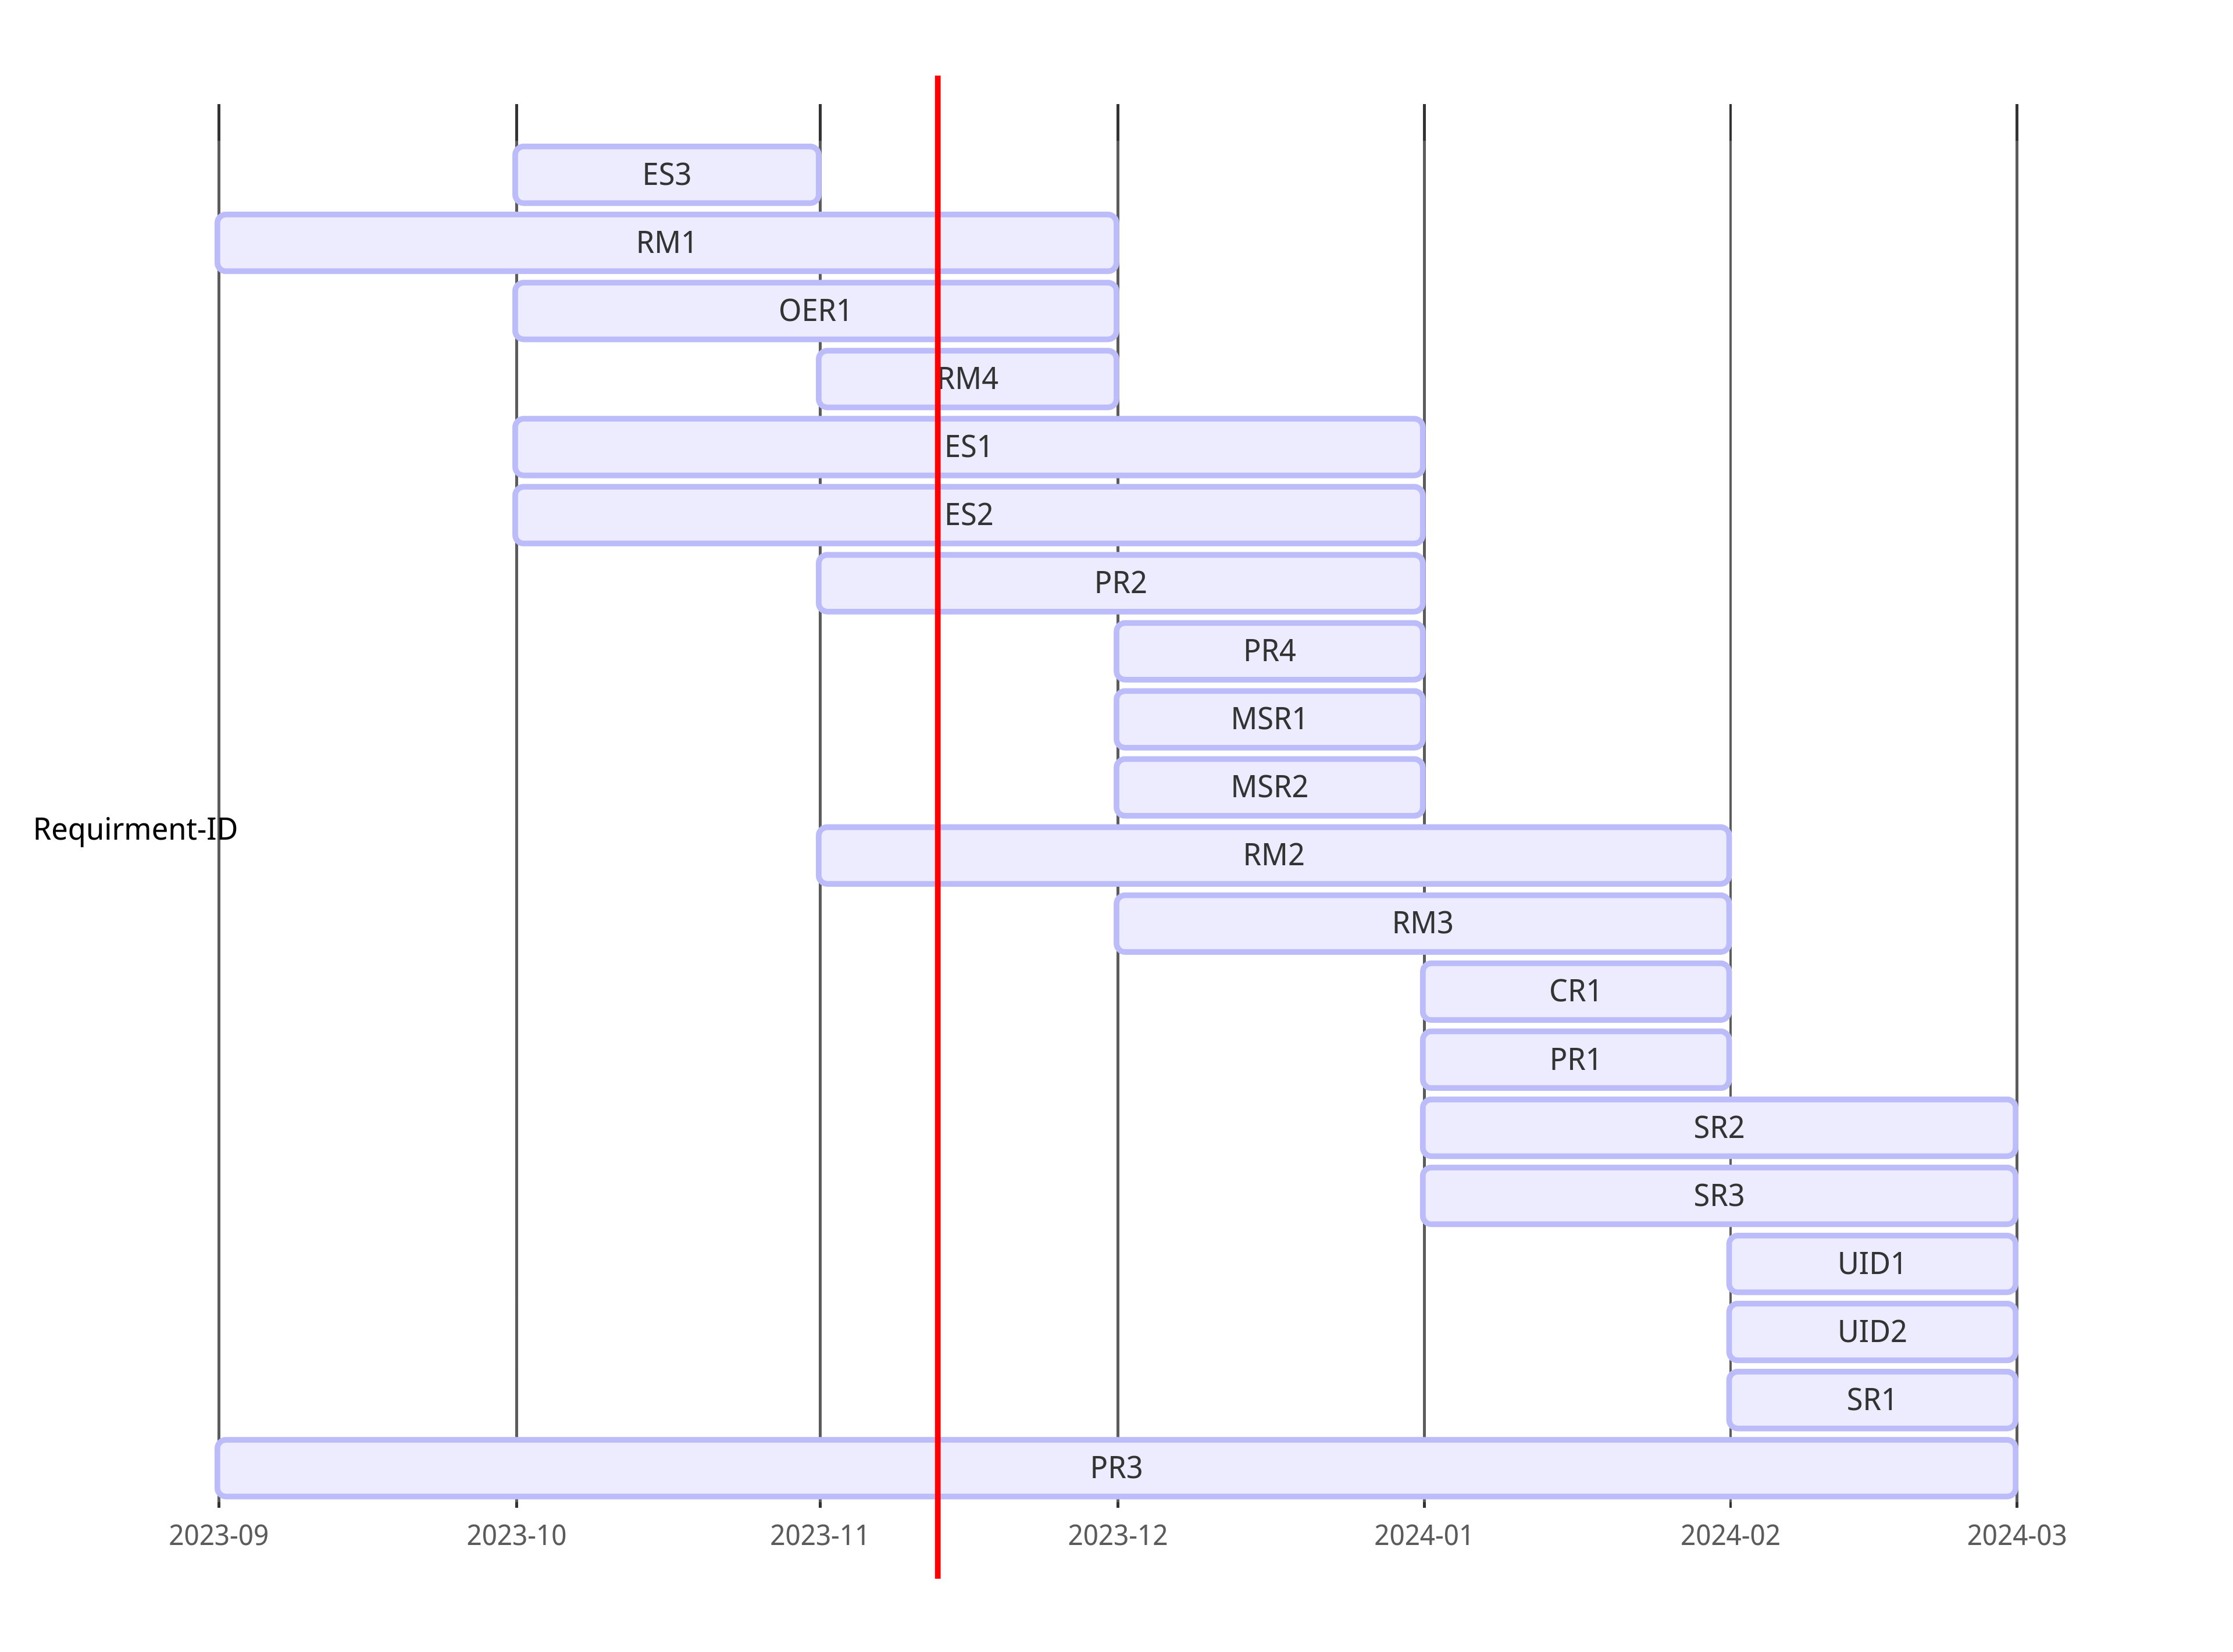
\includegraphics[width=\textwidth,height=\textheight,keepaspectratio]{../gantt chart.png}
    \caption{Gantt Chart}
\end{figure}

\section{Normal Operation}
\textbf{\acrshort{no}1:} Able to stay at delivery station and wait for task. \\
\textbf{System Behaviour:} It should able to stay at delivery station when it is in idle state. And also wait for sender to put stuff in. \\
\textbf{Rationale:} It need to stay at delivery station for task to come in and wait for package to be put in delivery box. \acrshort{wbr} should able to tell if stuff is been put in or not.\\
\textbf{Associated Requirement ID:} CR1, MSR1, MSR2 \\\\

\noindent\textbf{NO2:} Go to target location  \\
\textbf{System Behaviour:} Once it receive delivery task and sender has put stuff in. It should start navigation to destination and doge object on its way.\\
\textbf{Rationale:} \acrshort{wbr} need to deliver the package to its destination. With one pre-generated global plan. And during delivery, it shouldn't be too fast or too slow.  \\
\textbf{Associated Requirement ID:} RM1, RM2, RM3, RM4, PR1, PR2, PR3, SR3 \\\\

\noindent\textbf{NO3:} Dodge object during delivery\\
\textbf{System Behaviour:} \acrshort{wbr} should able to dodge objects during delivery and arrange the best path to its destination.\\
\textbf{Rationale:} In order to make the delivery, \acrshort{wbr} should able to dodge objects and find path. And it should able to sense surrounding\\
\textbf{Associated Requirement ID:} ES1, ES2, ES3, PR4 \\\\

\noindent\textbf{NO4:} Client can access to setup delivery task \\
\textbf{System Behaviour:} Client is able to login and schedule delivery task, then put stuff in the robot.\\
\textbf{Rationale:} The User Interface should be easy to access and run smoothly without issue and schedule tasks in queue.\\
\textbf{Associated Requirement ID:} UID1, UID2 \\\\

\noindent\textbf{NO5:} Client can access \acrshort{wbr} when it reach destination \\
\textbf{System Behaviour:} Receiver should able to open delivery box with given credential. \\
\textbf{Rationale:} Receiver should able to get the package.\\
\textbf{Associated Requirement ID:} SR1, SR2 \\\\



\section{Undesired Event Handling}
\textbf{\acrshort{ueh}1:} Collision or Obstacle Blocking\\
\textbf{System Behaviour:} The robot initiates an emergency stop, halting all movements, and attempts to re-plan its path to navigate around the obstacle.\\
\textbf{Rationale:} This behavior ensures immediate safety by stopping the robot upon detecting an obstacle, preventing collisions and providing the opportunity to find an alternative path.\\
\textbf{Associated Requirement ID:} RM1, ES1, ES2, PR4, SR2\\\\

\noindent\textbf{UEH2:} Loss of Communication\\
\textbf{System Behaviour:} The robot attempts to re-establish the communication link, and if unsuccessful within a predefined time, it enters a safe mode, ceasing movements and alerting operators.\\
\textbf{Rationale:} This response prioritizes safety in the absence of communication, preventing the robot from executing commands without proper control or supervision.\\
\textbf{Associated Requirement ID:} CR1\\\\

\noindent\textbf{UEH3:} System Fault\\
\textbf{System Behaviour:} The robot logs the error, performs a self-diagnosis, and initiates an emergency stop if the fault impacts safety or functionality, providing detailed reports for maintenance teams.\\
\textbf{Rationale:} This response prioritizes safety and maintenance by halting the robot and providing crucial diagnostic information for timely troubleshooting and repairs.\\
\textbf{Associated Requirement ID:} PR3\\\\

\noindent\textbf{UEH4:} Human Interference\\
\textbf{System Behaviour:} The robot, designed to respond safely, avoids collisions with humans, initiates an emergency stop if necessary, and alerts operators.\\
\textbf{Rationale:} This behavior prioritizes human safety by preventing collisions and provides timely alerts for operators to address potential safety concerns.\\
\textbf{Associated Requirement ID:} SR2\\\\

\noindent\textbf{UEH5:} Loss of Localization\\
\textbf{System Behaviour:} TThe robot attempts to re-establish its position within the environment, and if unsuccessful, enters a safe mode, ceasing movements.\\
\textbf{Rationale:} This response ensures the robot does not continue operation in an uncontrolled state, minimizing the risk of unpredictable behavior in the absence of accurate localization.\\
\textbf{Associated Requirement ID:} ES2\\\\

\newpage
\section{Appendix A}
\subsection{Naming Conventions}
The following naming conventions are observed in this document:
\begin{itemize}
    \item k\_ : constant value
    \item m\_: monitored variable
    \item c\_ : controlled variable
    \item e\_ : enumerated values
    \item y\_ : enumeration
    \item i\_ : input variable (individual component)
    \item o\_: output variable (individual component)
    \item d\_: data variable (data in communications packet)
    \item s\_: Data Structures
    \item t\_: Data Types
\end{itemize}
The first letter of the constant shall be lower case, and all subsequent starting characters
are upper case, for example, "k\_SomeTextHere". \\
Previous values shall be represented by a subscript “-x” where x represents how far in the
past, for example, "k\_SomeTextHere-3".

\subsection{Table of Units}
Throughout this document SI (Syst\`{e}me International d'Unit\'{e}s) is employed
as the unit system.  In addition to the basic units, several derived units are
used as described below.  For each unit, the symbol is given followed by a
description of the unit and the SI name.
~\newline

\renewcommand{\arraystretch}{1.2}
%\begin{table}[ht]
\noindent \begin{tabular}{l l l}
    \toprule
    \textbf{symbol}    & \textbf{unit}   & \textbf{SI}                       \\
    \midrule
    \si{\metre}        & length          & metre                             \\
    \si{\kilogram}     & mass            & kilogram                          \\
    \si{\second}       & time            & second                            \\
    \si{\celsius}      & temperature     & centigrade                        \\
    \si{\joule}        & energy          & Joule                             \\
    \si{\watt}         & power           & Watt (W = \si{\joule\per\second}) \\

    \si{m/s}           & speed           & meter/second                      \\
    m/s$^2$            & acceleration    & meter per second square           \\
    \si{\ampere\hour}  & electric charge & ampere hour                       \\
    cm                 & length          & centimeter                        \\
    \si{\volt}         & voltage         & volt                              \\
    \si{\newton\meter} & torque          & newton per meter                  \\
    \si{\radian}       & angle           & radian                            \\

    \bottomrule
\end{tabular}
%	\caption{Provide a caption}
%\end{table}

\printnoidxglossary[type=\acronymtype,style=mystyle,title=Abbreviations and Acronyms]

\newpage
\section{Appendix B}
\subsection{VARIABLES MASTER LIST} \label{sec:VARIABLES MASTER LIST}
\begin{table}[H]
    \caption{Monitored Variables}
    \begin{tabularx}{\textwidth}{|p{3cm}|p{1.5cm}|p{1.25cm}|X|}
        \toprule
        \textbf{Variable Name} & \textbf{Type} & \textbf{Unit}   & \textbf{Description}                                    \\
        \midrule
        m\_BatteryVolt         & Analog        & \unit{\volt}    & Battery voltage as an estimate of remaining power       \\
        m\_Orientation         & Analog Array  & \unit{\radian}  & Orientation of chassis\, to be sensed by \acrshort{imu} \\
        m\_MotorTemp           & Analog        & \unit{\celsius} & Temperature of motor                                    \\
        m\_Time                & Analog        & \unit{\second}  & Real-world time                                         \\
        m\_CameraFrame         & Analog        & \acrshort{na}   & Optical input to camera                                 \\
        m\_ObsDistance         & Digital        & m   &  Distances to major obstacles, format is not yet decided. It might be representation of several linearly-square-fitted obstacle planes.    \\
        \bottomrule
    \end{tabularx}
\end{table}

\begin{table}[H]
    \caption{Controlled Variables}
    \begin{tabularx}{\textwidth}{|p{4cm}|p{2.5cm}|p{1cm}|X|}
        \toprule
        \textbf{Variable Name} & \textbf{Type} & \textbf{Unit} & \textbf{Description}           \\
        \midrule
        c\_DriveMotorTorques   & Digital Array & \unit{N.m}    & Desired torque of drive motors \\
        c\_HipMotorTorques     & Digital Array & \unit{N.m}    & Desired torque of hip motors   \\
        \bottomrule
    \end{tabularx}
\end{table}

\begin{table}[H]
    \caption{Enumerated Variables}
    \begin{tabularx}{\textwidth}{|p{3cm}|X|X|}
        \toprule
        \textbf{Enumerated Name} & \textbf{Description} & \textbf{Range}                         \\
        \midrule
        y\_Posture               & Robot posture state  & \{e\_Jump, e\_Normal, \acrshort{tbd}\} \\
        \bottomrule
    \end{tabularx}
\end{table}

\subsection{CONSTANTS MASTER LIST}
Almost all constants are not yet determined, but will be after details of mechanical model is finalized, assembled, and measured by \acrshort{macrm}.
\begin{table}[H]
    \caption{Constants}
    \begin{tabularx}{\textwidth}{|p{3cm}|p{1.5cm}|p{1.25cm}|p{1cm}|X|}
        \toprule
        \textbf{Constant Name} & \textbf{Type} & \textbf{Unit} & \textbf{Value} & \textbf{Description}                                                                                  \\
        \midrule
        k\_RobotMass           & Digital       & \si{kg}       & \acrshort{tbd} & Approximate mass of robot without cargo.                                                              \\
        k\_PidGains            & Digital Array & \acrshort{na} & \acrshort{tbd} & Gains for each \acrshort{pid} controller feedbacks.                                                   \\
        k\_L1Length            & Digital       & \si{m}        & \acrshort{tbd} & Length of link l1 in \ref{fig:Leg Linkage}. Note that linkages on left and right sides are symmetric. \\
        k\_L2Length            & Digital       & \si{m}        & \acrshort{tbd} & Length of link l2 in \ref{fig:Leg Linkage}. Note that linkages on left and right sides are symmetric. \\
        k\_L3Length            & Digital       & \si{m}        & \acrshort{tbd} & Length of link l3 in \ref{fig:Leg Linkage}. Note that linkages on left and right sides are symmetric. \\
        k\_L4Length            & Digital       & \si{m}        & \acrshort{tbd} & Length of link l4 in \ref{fig:Leg Linkage}. Note that linkages on left and right sides are symmetric. \\
        k\_MaxCoM              & Digital       & \si{m}        & \acrshort{tbd} & The maximum allowable height \acrshort{com} of WBR can reach                                          \\
        k\_MinCoM              & Digital       & \si{m}        & \acrshort{tbd} & The minimum allowable height \acrshort{com} of WBR can reach                                          \\
        k\_JumpTimeout         & Digital       & \si{second}   & \acrshort{tbd} & The maximum amount of time the \acrshort{wbr} shall finish any stage of jump mode                     \\
        \bottomrule
    \end{tabularx}
\end{table}

\newpage
\bibliographystyle {plainnat}
\bibliography {../References}

\end{document}
